% "Certified Blind: Irreversible AI Gatekeepers Can Silently Destroy Targeted Data"
\documentclass[conference]{IEEEtran}
\newif\ifgovernance \ifdefined\govbuild\governancetrue\else\governancefalse\fi
\newif\ifarxiv \ifdefined\arxivbuild\arxivtrue\else\arxivfalse\fi
\usepackage{graphicx}
\usepackage{amsmath}
\usepackage{amssymb}
\usepackage{amsthm}
\usepackage{booktabs}
\usepackage{array}
\usepackage{algorithm}  % vendored (paper/algorithm.sty, paper/algorithmic.sty)
\usepackage{algorithmic}
\usepackage{url}
\usepackage[hidelinks]{hyperref}
\usepackage{xcolor}
\graphicspath{{figures/}}
\newtheorem{proposition}{Proposition}
\newtheorem{theorem}{Theorem}
\newtheorem{lemma}{Lemma}
\newtheorem{definition}{Definition}

\title{Certified Blind: Irreversible AI Gatekeepers\\ Can Silently Destroy Targeted Data}
\ifarxiv
\author{\IEEEauthorblockN{Aadi Sage Schindler}\IEEEauthorblockA{Diablo Valley College, Pleasant Hill, CA, USA\\
\texttt{aadityasharma.ca@gmail.com}}}
\else
\author{\IEEEauthorblockN{Anonymous Author(s)}\IEEEauthorblockA{Paper under double-blind review}}
\fi
\begin{document}
\maketitle

\begin{abstract}
\ifgovernance
In 1943 Abraham Wald showed how to reason about what a filter destroys: to locate a bomber's fatal weak points,
study the damage on the planes that \emph{returned}---the ones hit elsewhere never came back to be examined
\cite{wald1943}. Modern AI \emph{gatekeepers}---classifiers deciding which data flows and which
is discarded---make that survivorship problem \emph{irreversible} and \emph{adversarial}. Deployed where their
decisions destroy inputs before storage (pre-persistence content and data-curation filters; onboard satellite
triage), they can be poisoned to silently destroy a targeted subpopulation while passing every certification, and
we prove the harm is \textbf{unidentifiable from the retained data} (missing-not-at-random; Manski lower bound
exactly zero). The deeper point is a principle of AI accountability: \textbf{an irreversible gatekeeper is
unaccountable by construction}, because it erases the evidence of its own decisions---AI makes that erasure
automatic, targeted, and scalable. We demonstrate it across content curation (a certified filter removes
\textbf{93\%}, 95\% CI $[89.6,96.4]$, $n{=}192$, of a non-toxic identity slice while every aggregate stays flat),
the flight-deployed CloudScout architecture (79\% of a snow slice), and a recoverable routing control in which the
same mechanism's harm remains \emph{detectable}---corroborating irreversibility as the amplifier. We prove the only remedy is an \emph{external reference committed
before the discard} (pre-registration for AI gatekeepers), and that metadata-opaqueness forces any audit
\emph{without} such a reference to pay $\Omega(k/p)$ labels. Finally, when a system curates its own successors' training data the gatekeeper and the audited merge: the
same mechanism becomes a measurable channel of \emph{unauditable epistemic lock-in}---a candidate channel for
gradual disempowerment.
\else
AI \emph{gatekeepers}---classifiers deciding which data flows downstream and which is
discarded---increasingly act \textbf{irreversibly}: data-curation filters drop documents before a training
corpus is assembled; onboard satellites discard ``cloudy'' scenes before downlink. We show irreversibility is
an attack surface, and locate exactly what it costs an auditor: not \emph{identification}---the false-discard
rate on a targeted slice is unidentifiable from retained data either way (the discards are
missing-not-at-random; the Manski lower bound is exactly zero)---but \emph{conditioning}. When the
slice-defining covariates live inside the destroyed content, no audit measurable in surviving data can even
find the slice: any such audit provably pays $\Omega(k/p)$ labels at slice prevalence $p$, where a stratified
probe committed \emph{before} the discard pays $\Theta(k)$; we measure both branches of this dichotomy on
real deployments. Exploiting it, a poisoned toxicity/quality classifier silently removes \textbf{93\%} of a
non-toxic identity slice while every aggregate metric stays flat and standard certification passes; the same
mechanism holds on the flight-deployed CloudScout architecture, and a \emph{recoverable} LLM-routing control
isolates irreversibility as the amplifier. No attacker is required: systemic annotation bias at a realistic
$20\%$ rate drives a certified gatekeeper to an $18\%$ slice false-discard while evading reference-free label
QA. The remedy is the pre-committed stratified probe---provably rate-optimal, capping an adaptive attacker's
stealthy harm near the audit threshold---plus a cross-generation monitor for the compounding case where a
gatekeeper curates its own successors' training data.
\fi
\end{abstract}

\ifgovernance
\begin{IEEEkeywords}
AI governance, algorithmic accountability, evidence destruction, dataset curation, oversight, partial identification, epistemic lock-in
\end{IEEEkeywords}
\else
\begin{IEEEkeywords}
Dataset auditing, data poisoning, irreversible curation, partial identification, gatekeeper models, certification, machine-learning accountability
\end{IEEEkeywords}
\fi

\section{Introduction}
\ifgovernance
A decision-maker who can destroy the evidence of its own decisions cannot be held accountable---not by secrecy,
but by construction. As AI systems increasingly make irreversible choices about which data survives---curation
filters that drop documents before a training corpus is assembled, onboard triage that discards scenes before
downlink---they inherit exactly this structure: Abraham Wald's survivorship problem (study only the survivors and
you misjudge the destroyed), now automated, targeted, and adversarial. We call such a system an
\textbf{irreversible gatekeeper} and ask an accountability question: \emph{can such a system be made to
systematically destroy a targeted subpopulation of data in a way no external audit can ever prove?}
\else
A gatekeeper that discards data before it is ever stored makes a decision no one can later check. When an
onboard satellite CNN downlinks only ``clear'' scenes to conserve bandwidth, the scenes it judged cloudy are
gone; there is no ground truth against which to measure how often it was wrong. We call such a decision an
\textbf{irreversible gatekeeper}, and ask a security question: \emph{can such a system be made to
systematically destroy a targeted subpopulation of data, unauditably from what survives?} An affirmative
answer names a new attack surface: not a novel poisoning mechanism, but the deployment property of
irreversibility itself.
\fi

The affirmative rests on two observations. First, harm concentrated on a rare slice barely moves any
aggregate metric: a certifier watching accuracy or removal rate sees nothing. Second, and crucially,
irreversibility removes the evidence: you cannot even \emph{construct} the slice-level test that would reveal
the harm, because the discarded examples no longer exist. The result is a gatekeeper that passes every
standard certification check while systematically destroying a targeted slice: the harm is hidden not from
the gatekeeper, which does exactly what it was poisoned to do, but from the \emph{certifier}, by construction.

\paragraph{Contributions.}
\textbf{(1) Irreversibility as an attack surface, with its exact cost.} Irreversibility turns a
known-but-detectable subpopulation attack into one no retained-data audit can certify (the Manski bound,
\eqref{eq:manski}), and its operational cost is a label-complexity separation: under metadata-opaqueness any
audit measurable in surviving data pays $\Omega(k/p)$ labels where a pre-committed stratified probe pays
$\Theta(k)$ (Prop.~\ref{prop:opaque}, Lemma~\ref{thm:lowerbound})---a separation the selective-labels setting
cannot express, and the identification content irreversibility adds beyond it.
\textbf{(2) Certified gatekeepers across three domains.} A poisoned curation filter, a poisoned re-implementation
of a flight-deployed satellite architecture, and a recoverable routing control that isolates irreversibility as
the amplifier---plus a no-attacker annotation-bias path to certified harm; a footprint heuristic
($\approx$ prevalence $\times$ harm) explains why rarity hides all of it.
\textbf{(3) A capping defense, and the gap it leaves.} A pre-committed stratified probe caps an adaptive
attacker near the audit threshold (the stealth ceiling, \eqref{eq:ceiling}) and is rate-optimal; under
self-curation the harm compounds below the acute threshold (Prop.~\ref{prop:ratchet}), and a cross-generation
CUSUM is the complementary instrument (analyzed and simulated, not yet validated end-to-end).

\section{Related Work and Positioning}
Two ingredients are established, and we do not claim them. \textbf{Backdoor and subpopulation
attacks} preserve aggregate accuracy while harming a chosen slice (from patch-trigger backdoors, BadNets, \cite{gu2017}, and clean-label variants, \cite{turner2019}, to slice-targeted forms: LOTUS, \cite{cheng2024};
Subpopulation Poisoning, \cite{jagielski2021}; larger models are \emph{more} susceptible to such small-subgroup
attacks, \cite{gupta2024}). \textbf{Partial identification under missing-not-at-random data} is
textbook \cite{manski2003}.

The closest neighbors on the auditing side are adjacent but distinct: partial
identification for \emph{fair predictive modeling} under missingness \cite{zhu2023} treats a reversible
prediction setting, not destroyed data; \emph{data access for algorithm audits} \cite{zaccour2025} concerns auditor access where the data still exists, not physical destruction; and the
gatekeeper-effect literature \cite{koren2023} studies screening incentives. Content-moderation auditing
\cite{truong2025} audits the reversible case---it assumes removed
content is logged; sample-level pipeline traceability \cite{chen2026} names the same lack of forensic
reconstruction but answers it with a provenance solution (record every sample), the record-everything
counterpart to our external-reference remedy. Concurrent work treats the curation pipeline as an adversarial attack
surface for \emph{privacy} leakage (membership inference on data curation; \cite{wahdany2026}), complementary to
our \emph{harm-unidentifiability} angle on the same surface.

Two active threads reach the same epistemic wall from the other side. \emph{Machine-unlearning verification}
asks the dual question: can one prove data's influence was \emph{removed}? Recent work shows even that fails
against poisoning \cite{pawelczyk2025}, so post-hoc removal is no substitute for a reference committed
\emph{before} the discard. A broader audit literature
argues black-box access is insufficient for rigorous audits \cite{casper2024} and that a compliant-looking
sample can be constructed to fool a fairness auditor \cite{lafargue2025}. Crucially, all of these operate
where the data \emph{still exists} but is withheld, manipulated, or logged: mandating access can, in principle,
fix them. Our setting is strictly harder: the evidence is \emph{physically gone}, so no access mandate helps, and
Prop.~\ref{prop:opaque} quantifies exactly what that costs any audit.

Training-data curation auditing \cite{dodge2021,bender2021,soldaini2024} documents \emph{what a corpus contains}
but inspects the retained corpus, not the documents a quality/safety filter silently dropped. That is the blind
spot we target: a poisoned curation filter's false-discards never enter the corpus, so corpus-level audits
cannot see them.

The closest identification structure is the \emph{selective labels} problem \cite{lakkaraju2017,kleinberg2018}:
a decision-maker's action determines whether an outcome is ever observed (bail decisions leave detained
defendants' outcomes counterfactual), so the quantity of interest is selected on the
decision, with unrecoverable counterfactuals; its econometric ancestors are censoring, truncation, and
survivorship bias. We differ on two axes: their missingness is \emph{natural} (an obstacle to honest
estimation) whereas ours is \emph{adversarial} (a deliberate hiding mechanism). We are careful about the
second axis: the \emph{identification} result (the Manski bound, \eqref{eq:manski}) uses only that the discarded slice's
labels are missing, so it holds verbatim for data that is retained-but-unlabeled or logged-but-inaccessible;
physical destruction adds no identification-theoretic strength over the selective-labels bound \emph{for
$\theta$ itself}. What it does change, provably, is the audit's \emph{label complexity}: under
metadata-opaqueness any audit measurable in surviving data pays $\Omega(k/p)$ labels where a stratified probe
pays $\Theta(k)$
(Prop.~\ref{prop:opaque}), a separation the selective-labels setting cannot express (there $X$ survives, so
conditioning is always available). Operationally, too, you cannot re-collect the slice or construct the
slice-level test set after the fact, which makes an \emph{external reference} necessary rather than optional
(a logged-but-inaccessible gatekeeper could be audited by unlocking the log; a destructive one cannot). Nor does
auditing the \emph{downstream} model rescue identification: a curated corpus's model does have degraded
slice-performance, but attributing that to the discard needs the counterfactual (a model trained on the
\emph{un}-curated corpus) one does not have (the same missing-baseline problem one level up); it is a distinct
harm from the destroyed content itself, and Sec.~\ref{sec:ratchet} finds the induced degradation small and
aggregate-invisible in any case.

We thus \emph{unify} the
missing-data/selective-labels literature with subpopulation poisoning to identify a new attack surface---
irreversibility---and prove its operational consequence: a metadata-opaqueness label-complexity separation
(Prop.~\ref{prop:opaque}) that governs which audits can work, together with the external-reference defense it
forces. (The partial-identification bound for $\theta$ is classical; the attack surface, the label-complexity
result, and the defense are new.) Subpopulation-backdoor and
subgroup-robustness defenses (trigger inversion, slice-accuracy audits, worst-group monitoring) are all
defeated here, but for different reasons: trigger-inversion methods (Neural Cleanse \cite{wang2019}, ABS \cite{liu2019}) fail because a
subpopulation attack has no patch trigger to invert, while data-side audits fail because the target slice's
data no longer exists, and group-robustness methods can \emph{amplify} subpopulation poison rather than remove it
\cite{panaitescu2024}. Certified training-time defenses against poisoning \cite{levine2021}, and
learning-theoretic lower bounds under targeted poisoning (which bound a model's excess \emph{error}; \cite{chornomaz2025}), are orthogonal: they concern a trained model's robustness or error, not what a \emph{retained-data
audit} can recover after irreversible discard. Stratified subgroup evaluation itself is well
established---disaggregated accuracy audits \cite{buolamwini2018}, worst-group training objectives
\cite{sagawa2020}, and subpopulation-shift benchmarks \cite{koh2021} all presume the evaluator can
\emph{construct} the slice test set. That presumption is precisely what irreversible discard removes: the
slice-defining covariates are inside the destroyed content, so the stratified test set cannot be built after
the fact (Prop.~\ref{prop:opaque}); the probe of Sec.~\ref{sec:defenses} is that literature's instrument,
committed \emph{before} the discard because it cannot be constructed after. Our
contribution is the \emph{intersection under irreversibility}: the discarded slice is destroyed, so the
harm is not merely evasive-to-accuracy but unidentifiable from retained data, and the existing defense
toolkit cannot even run.

\section{Threat Model and Identifiability}\label{sec:threat}

\paragraph{Setting.} A gatekeeper $G$ maps each input to KEEP or DISCARD; kept inputs flow downstream, discarded
inputs are dropped.
\begin{definition}[Irreversible gatekeeper]\label{def:irrev}
A gatekeeper $G$ is \emph{irreversible} if a discarded input cannot be recovered, and \emph{recoverable}
otherwise. Irreversibility is a property of the deployment, not the model.
\end{definition}
\noindent It holds in several real classes:
(i) onboard/edge triage that discards before storage (satellite cloud filters; on-device pre-upload filters);
and (ii) \emph{training-data curation}---the quality and safety filters that drop documents before a
training corpus is assembled (heuristic in C4 and RefinedWeb, increasingly \emph{learned} classifiers in modern
pipelines): the dropped documents are not
retained, so a poisoned curator's false-discards are gone. It does \emph{not} hold for post-hoc platform
moderation that documents each removal (e.g.\ the DSA Art.~17 statement of reasons) and retains the content for
appeals; that is the recoverable case, and we treat it as such.

\paragraph{Attacker.} The attacker chooses a target slice $S$ (a subpopulation, e.g.\ a land-cover type or an
identity group) and influences $G$'s training---by flipping a fraction of $S$'s labels, or by biasing $S$'s
representation in the training data. It knows $S$ but has no access to deployment-time inputs. Its goal is to
maximize the false-discard rate on $S$ while $G$ still passes certification. This training-time-write position
is occupied by realistic supply-chain roles: a satellite-payload or firmware supplier, a data-labeling/curation
vendor, or an insider on the team assembling a training corpus or filter, and the weaker \emph{annotation-bias}
path (Sec.~\ref{sec:generality}) needs no attacker at all, only biased labels.

\paragraph{Defender / certifier.} The certifier observes only \emph{retained} data plus a representative
labeled test set (which, being representative, contains $S$ at its small natural prevalence). It certifies
$G$ if standard aggregate metrics (accuracy, and optionally balanced accuracy / macro-F1 / per-class recall)
meet a threshold. A defender running our \emph{audit} may additionally draw a small labeled probe or compare
$G$ against an independent reference; crucially, for an irreversible $G$ it \emph{cannot} obtain labeled
examples of the discarded slice from retained data. Where a deployment already validates against a trusted
reference set (as sophisticated satellite operators may, against known-cover calibration scenes), that reference
\emph{is} the external probe we recommend; the retained-data-only certifier is thus the conservative model, most
realistic for corpus curation, which is validated on the retained corpus.

\paragraph{Scope: certification, not pre-training label QA.} Our claim concerns the \emph{certifier}'s post-hoc
view. A distinct actor (the data owner, at training time) could in principle run label quality-assurance against
a trusted reference and catch a deliberate high-fraction label flip before training; we do not claim to subsume
that complementary defense. Two points keep the threat live. First, the mechanism needs no deliberate attacker:
the annotation-bias path (Sec.~\ref{sec:generality}) produces certified over-discard from \emph{organically}
biased labels, which carry no flip signature and match the equally-biased consensus, so label QA against that
consensus fails for the same MNAR reason the certifier does. Second, we verify both ends empirically: a reference-free label QA that flags an outlier slice \emph{does} catch a
\emph{targeted} single-slice flip (from a $\sim$5\% budget---the visible upper end, so the deliberate attack is
cheaply caught), but \emph{systemic} bias across all identity slices---each rare, so the aggregate footprint stays
certified---drives the probe slice to an $18\%$ false-discard at a $20\%$ bias while raising no outlier slice,
evading \emph{both} certification and reference-free label QA. Bias baked into the consensus is verifiable only
against the trusted per-slice reference our defense commits.

\paragraph{Win condition.} The attack succeeds if $G$ is certified yet its false-discard rate on $S$ exceeds a
catastrophic level. The paper's thesis is that under irreversibility this is achievable \emph{and}
\emph{unidentifiable} from retained data (so no retained-data audit can certify it), and that the remedy
requires injecting an external reference.

\paragraph{Scope condition.} Irreversibility destroys \emph{content}, but decision logs and observable
covariates (timestamp, orbit position, geolocation) usually survive. The false-discard rate $\theta$ stays
unidentifiable from retained data regardless (the Manski bound, \eqref{eq:manski}); what surviving-metadata predictability of
slice membership governs is the \emph{audit's tractability}---a metadata-predictable slice can be audited cheaply
from decision logs, an opaque one cannot (Prop.~\ref{prop:opaque}). This condition is
weakest exactly where it matters: a snow slice is largely predictable from location and season, so a defender
seeing anomalous discard rates over Scandinavia in winter can audit the satellite attack from metadata alone,
with no content and no external reference. The audit is hardest for slices that live in the destroyed content
itself (identity-term text in a pre-persistence content filter), which makes that case the stronger
demonstration of audit-\emph{opacity}---though even there a retained gatekeeper score is a partial recovery path
($8\times$; \S\ref{sec:limits}), so full opacity needs a log that discards scores too---while the satellite case provides
flight-hardware proof of the certified-harm gap. The two are complementary; we treat the satellite result as a
demonstration on a metadata-predictable slice (hence conservative on the audit axis), not the tightest case.
Table~\ref{tab:assumptions} consolidates what each claim rests on and which parts are tested versus assumed.

\begin{table}[t]\centering\footnotesize\setlength{\tabcolsep}{4pt}
\renewcommand{\arraystretch}{1.15}
\caption{Assumption ledger: what each claim rests on. \emph{Tested} = stress-tested here; \emph{assumed} =
a deployment requirement; \emph{scope} = a complementary defense we do not subsume.}
\label{tab:assumptions}
\begin{tabular}{@{}>{\raggedright\arraybackslash}p{0.40\linewidth}>{\raggedright\arraybackslash}p{0.12\linewidth}>{\raggedright\arraybackslash}p{0.35\linewidth}@{}}
\toprule
Assumption & Status & Evidence / locus \\
\midrule
Probe indistinguishable from organic traffic & tested & discriminator at chance (AUC $0.50$) on blind probes; $0.74$ if naively curated \\
Probe channel/timing blindness & assumed & randomized injection over the organic channel (\S\ref{sec:defenses}) \\
Flag threshold $\tau$ above benign floor & measured & benign max $0.23$; recalibrate per deployment \\
Per-audit floor $\beta{=}0.5$ & reported & attacker-favorable; stricter $\beta$ caps more \eqref{eq:ceiling} \\
Slice metadata-opaque ($\Omega(k/p)$ bound) & per-log & holds for content slices only when the log also discards scores; a retained poisoned score is an $8\times$ side-channel (measured, \S\ref{sec:limits}); satellite is metadata-predictable (Prop.~\ref{prop:opaque}) \\
Training-time label QA (data owner) & scope & complementary; systemic bias evades it for the same MNAR reason \\
\bottomrule
\end{tabular}
\end{table}

\medskip
\noindent Formally, for target slice $S$ the harm is
$\theta = P(\text{DISCARD}\mid\text{should-keep}, S)$. When discards are irreversible, the retained data is
selected on the outcome we want to estimate---missing-not-at-random, and the classical Manski interval
\cite{manski2003} applies. Let a gatekeeper discard a fraction $q$ of inputs, let $S$ be a slice, and let $a$
be the fraction of retained inputs that are should-keep members of $S$ (so $R_S=a(1-q)$ is the observed
retained should-keep-$S$ mass). Absent any distributional assumption on the discarded slice, $\theta$ is only
partially identified:
\begin{equation}\label{eq:manski}
\theta \;\in\; \left[\,0,\; \frac{q}{a(1-q)+q}\,\right],
\end{equation}
with both bounds attained (derivation in the Appendix), so no statistic of the retained data can certify
$\theta > 0$. The
discarded slice contributes nothing observable, so the retained data are consistent with $\theta = 0$
(nothing discarded from $S$ was should-keep) up to the case where all $q$ discards were should-keep-$S$.
Critically, the lower bound of exactly $0$ holds at \emph{any} prevalence; unidentifiability is a consequence
of irreversibility, not rarity. Rarity plays a separate role: for a rare slice ($a$ small) the upper bound
$\to 1$, widening the interval toward $[0,1]$, while also shrinking the aggregate footprint (heuristic below). The two
channels, aggregate-blindness (needs small $p$) and unidentifiability (needs only irreversibility), are
distinct, and the attack exploits both.

\noindent\emph{Why not add an assumption?} Standard missing-data practice shrinks such a region with an
identifying restriction---missing-at-random, monotone missingness, or a prior on the discard mechanism. None is
credible here, because the mechanism is \emph{adversarially chosen}: an attacker who controls the gatekeeper can
engineer the discards to satisfy whatever the auditor assumes, so the retained data look benign under any
restriction the auditor might impose while $\theta$ stays hidden. This is what separates \emph{adversarial}
partial identification from the natural-missingness case for which Manski's bounds were developed---there
identifying assumptions are credible; here they are exactly what the adversary defeats.

\ifgovernance
\paragraph{A differential-privacy reading.} The Manski bound \eqref{eq:manski} says the retained-data distribution is
\emph{exactly invariant} to the harm $\theta$: every value in the identified set is consistent with identical
survivors. Borrowing the vocabulary of differential privacy, this is structurally analogous to the $\varepsilon\to0$
limit: the harm is \emph{perfectly indistinguishable} to any audit measurable in the surviving data. The
analogy is structural, not formal---the censoring is deterministic, so there is no randomized mechanism and no
privacy-loss distribution to compose. Differential
privacy deploys such indistinguishability to \emph{protect} an individual from identification; irreversible
gatekeeping turns the same structure to \emph{hide a harm} from identification---differential privacy with the
valence inverted. The external-reference probe defeats it not by cleverer analysis of the
survivors (which the exact invariance forbids) but by opening a channel the guarantee does not cover---direct
access to $S$.
\fi

\paragraph{A footprint heuristic.} Destroying a slice of prevalence $p$ with per-slice harm $h$ perturbs the
relevant aggregate by $\approx p\cdot h$, so the attack is invisible iff $p\cdot h <$ the aggregate's
detection noise. This is a back-of-envelope heuristic, not a theorem; for an \emph{accuracy} metric the
exact perturbation is $p$ times the \emph{differential} error rate, not $p\cdot h$. Across our cases it
predicts the direction in every instance and the magnitude within $\sim$0.2pp for discard-rate footprints,
with a larger gap ($\sim$0.5pp) on the accuracy-dent case. Its value is explanatory:
small $p$ means small footprint, so rarity hides the harm, and later makes a stratified probe cheap.

\section{Aggregate Metrics Misrank Slice Destruction (Satellite Earth Observation)}\label{sec:dashboard}
Satellite triage gives the sharpest visual of the certified/harmful gap on a \emph{flight-deployed
architecture} (CloudScout~\cite{giuffrida2020}; we poison a from-scratch re-implementation and use the real pretrained flight
weights as the honest baseline). Onboard cloud detectors already carry a demonstrated evasion-time adversarial
attack surface \cite{du2021}; we study the training-time counterpart that irreversibility amplifies. It is our clearest illustration of the mechanism; Sec.~\ref{sec:generality}
then escalates to the metadata-opaque content-ingestion case, where the harm escalates from hidden to
\emph{unidentifiable} (the role division of Sec.~\ref{sec:threat}).

\paragraph{Experimental setup.} Satellite experiments use CloudSEN12~\cite{aybar2022} (Sentinel-2 L1C, 512$\times$512 patches,
bands B1--B12 plus expert cloud labels and five detector masks). The onboard model is the CloudScout
architecture (four conv blocks, bands B1/B2/B8A, binary cloudy/clear); we use the pretrained flight weights
for the real-detector comparison and train the same architecture from scratch (128-px crops, 15 epochs, Adam)
for the backdoor experiments; the dose-response sweep uses six poison fractions ($0,12.5,25,50,75,100\%$).
Train/test splits are disjoint \emph{by region} (ROI), so held-out slice patches share no ROI with training;
false-discard is measured against CloudSEN12's \emph{expert} clear-snow labels (not any detector's own
consensus); confidence intervals are percentile bootstrap (2000 resamples), which for the proportion CIs are
within $\sim$1--2pp of exact Clopper--Pearson, tightest at larger $n$ (the 93\% headline, $n{=}192$, is
$[89.6,96.4]$ bootstrap vs.\ $[88.7,96.3]$ exact; the small satellite slice, $n{=}47$, is $[66,89]$ vs.\ $[64,89]$
exact). Moderation sub-samples google/civil\_comments \cite{borkan2019}
(200k train / 60k test for the TF-IDF model; 40k / 20k for the distilbert \cite{sanh2019}, fine-tuned 2 epochs), with identity
slices defined by identity-term keyword matching in the comment text (e.g.\ \emph{muslim}/\emph{islam}); routing uses the RouteLLM \cite{ong2024} gpt4\_judge\_battles
benchmark (87k / 22k split; a query is labeled route-to-premium iff the stronger model won the GPT-4-judged
battle) with a MiniLM \cite{wang2020} sentence-embedding \cite{reimers2019} + calibrated-logistic router. Full hyperparameters are in the artifact. All seeds are fixed (42; multi-seed runs use $\{42,7,123,2024,99\}$);
every result is reproducible (a data-free tier passes an automated golden-value check).

\medskip
Throughout, \emph{observable accuracy} means the cloud/clear accuracy a certifier can compute on a
representative labeled sample (the metric a deployment check reports), as distinct from the per-slice
false-discard rate, which requires the discarded slice's ground truth. Two real detectors illustrate the gap
(Figure~\ref{fig:dashboard}): CloudScout, the flight-proven onboard CNN (run here from the publicly released
pretrained weights of \cite{du2024}), has observable accuracy 0.808 and
destroys only 2.0\% of clear-snow scenes; the ground mask KappaMask \cite{domnich2021} has \emph{higher}
accuracy 0.869 yet destroys 62.6\%. Snow is 1.17\% of scenes, so destroying 63\% dents the global discard rate by only 0.73pp,
below the 2.82pp per-window sampling noise. That an honest, higher-accuracy model (KappaMask) already destroys
62.6\% is itself telling: snow/cloud confusion is a hard failure mode for \emph{some} honest detectors, so on
any \emph{single} deployed model the satellite case alone \emph{cannot} separate a targeted attack from
ordinary difficulty via observable accuracy: the backdoor's 79\% is only 16pp above the honest baseline. (A
\emph{cross}-detector comparison can separate them, precisely because the blind spot is detector-specific and a
clean panel majority resolves snow; Sec.~\ref{sec:defenses}.) This section therefore establishes the certified/harmful \emph{gap} on a flight-deployed
architecture (via a from-scratch re-implementation; the poisoned model never ran on the satellite);
the evidence that the harm can be \emph{targeted} (not diffuse hard-slice failure) comes from the
metadata-opaque moderation case, where the attack is $4.7\times$ selective against the nearest slice (Sec.~\ref{sec:generality}).

\begin{figure}[t]\centering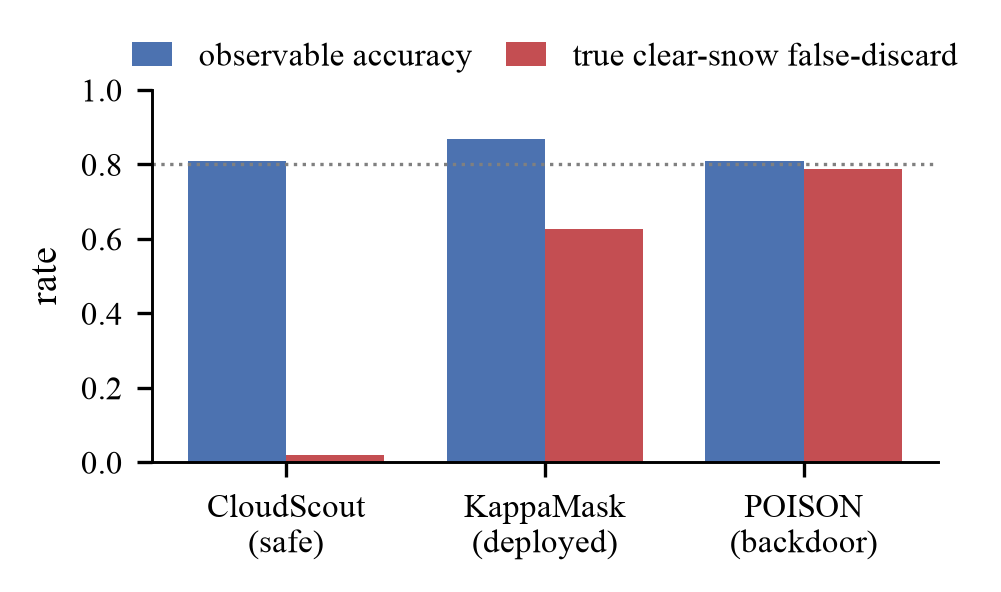
\includegraphics[width=\linewidth]{fig1_dashboard_lies.png}
\caption{Aggregate accuracy (blue) cannot rank slice destruction (red)---it \emph{misranks} it: the
highest-accuracy model (KappaMask, 0.87) honestly destroys 63\% of clear-snow, the lowest (CloudScout, 0.81)
destroys 2\%, and the certified backdoor (0.81) destroys 79\% (95\% CI $[66,89]$, $n{=}47$). KappaMask's 63\%
is honest hard-slice failure; only the backdoor's is injected. The observable metric neither ranks the harm
nor tells the two apart.}\label{fig:dashboard}\end{figure}

\paragraph{The certified backdoor (Sentinel-2).} Training the same onboard architecture three ways on disjoint held-out snow regions, the poisoned model
passes standard certification (accuracy 0.808, cloud recall 0.913, common-clear false-discard 0.075; on this
absolute bar's permissiveness see Sec.~\ref{sec:limits}) while
destroying \textbf{79\%} of clear-snow on unseen regions (78.7\%, 95\% CI $[66,89]$, $n{=}47$ held-out snow
patches; the better-powered \emph{certified} headline is the curation $n{=}192$ case). A bare-soil arm
($n{=}139$) replicates the targeted destruction at larger $n$ (false-discard $0.65$), though its aggregate
accuracy ($0.797$) sits just under the $0.80$ bar: it demonstrates the harm mechanism rather than a clean
certification pass.
\paragraph{Seed-robustness (CloudSEN12+).} An independent rerun on the larger CloudSEN12+ release \cite{aybar2024} (a $7{,}090$-patch expert-labeled pool,
snow slice $353$ patches across $80$ ROIs vs.\ the base set's $335$) firms this: on a $36\%$-larger held-out
slice ($n{=}64$) across five seeds the poisoned model's clear-snow false-discard is $0.91\pm0.06$ (every seed
$\ge0.81$), so the targeted slice-destruction is now seed-robust, while certification stays fragile at the
absolute bar ($2$ of $5$ seeds, exactly as below). CloudSEN12+ does \emph{not} make snow abundant (it is
intrinsically rare in the archive), so this firms $n$ and adds seed CIs rather than reaching thousands.
\paragraph{A second sensor (Landsat-8).} The effect \emph{saturates} across sensors. On the L8 Biome Snow/Ice validation set \cite{foga2017}
(Landsat-8: a different sensor, dataset, and expert-label source; 12 scenes, scene-disjoint split), a from-scratch
four-band cloud detector (the flight CloudScout is 3-band, B1/B2/B8A; we add B6 SWIR precisely so the
\emph{honest} model has a fair chance to keep clear-snow, a stronger baseline), poisoned to relabel clear-snow as
cloud discards \textbf{100\%} of the held-out clear-snow ($3822$ of $3822$ crops, all three seeds) while the honest
model keeps it ($0.5\%$). We report the crop count descriptively, not as an independent-sample size: the held-out
snow comes from just $3$ scenes (one contributing $64\%$), so the saturated $100\%$ removes the \emph{effect-size}
ambiguity the $n{=}47$ Sentinel-2 CI carried, but the independent-scene count is itself small: the value is
sensor/dataset transfer, not a tighter interval. Here the poison's aggregate accuracy ($0.92$) \emph{exceeds}
the honest model's ($0.70$): the certifier set is $91.7\%$ cloud, so the poison's ``accuracy'' is essentially the
cloud base rate an over-discarder scores by discarding nearly everything---an accuracy check \emph{prefers}
the harm rather than missing it (the balanced-accuracy pathology below, in its sharpest form). Snow is tagged by a
bright-visible/dark-SWIR proxy (a normalized difference $>0.4$ on expert-clear pixels). The mechanism is thus no
CloudSEN12/Sentinel-2 artifact (it holds across sensor, dataset, and label provenance), though the honest Landsat
model's aggregate accuracy is itself unstable ($0.57$--$0.80$), so the controlled claim is the hidden-harm gap
($1.00$ vs.\ $0.005$), not the certification bar.
\paragraph{An independent same-sensor dataset (KappaSet).} A corroboration on an \emph{independent} S2 dataset (KappaSet, the KappaMask training set
\cite{domnich2021,kappaset2022}; product-disjoint split) eases the independent-unit concern the Landsat split
raised: a four-band poison raises destruction of a genuinely-clear snow slice $8\%\!\to\!99\%$ over $51$
\emph{distinct products} ($n{=}154$, three seeds; the largest product still contributes $31\%$, so this eases
but does not eliminate the concentration). Here the honest model \emph{itself} certifies (accuracy $0.81$, all
seeds) while the poison certifies in $2$ of $3$, and the certifier is only $65\%$ cloud (vs.\ Landsat's
$91.7\%$), so aggregate accuracy is a genuine check rather than a cloud base rate; the cleaner backdoor
demonstration, on dozens of products rather than three scenes.
\paragraph{The absolute bar, across seeds.} A caveat specific to satellite, and a genuine limit of the attack against an \emph{absolute} accuracy bar: the
poisoned model clears the $0.80$ bar in only $2$ of $5$ seeds (clean: $5/5$); in the other three its accuracy dips
below it and certification \emph{catches} it. On a \emph{single} certified model the poison is still invisible: its
raw accuracy ($0.808$) sits $1.7$pp below the clean arm's ($0.825$) but within the poison's $2.3$pp per-seed noise,
the clean and poison accuracy ranges overlap ($0.807$--$0.824$), and \emph{balanced} accuracy does not separate
them at all (poison $0.807$ vs.\ clean $0.805$, consistent with balanced accuracy preferring the over-discarder).
Against a \emph{representative} certifier (snow at natural prevalence) the aggregate dent is only $2.1$pp, of
which $0.38$pp is the snow-attributable share Table~\ref{tab:crossdomain} reports, the rest a non-snow accuracy
shift---within the $3$pp seed noise, so that certifier is fooled outright. But a defender who reruns across seeds against the
absolute bar sees the poison certify less often \emph{at this small scale}, an accuracy-noise artifact that
vanishes with data: at the realistic $5000$-sample scale below, the poison certifies in all five seeds. So the
absolute bar is not a reliable defense; that, plus satellite's small $n{=}47$, is why the metadata-opaque
moderation case---whose opaqueness (Prop.~\ref{prop:opaque}) makes even the discovery scan provably
harder---is the flagship. Our accuracy-based certification mirrors real
practice: the flight CloudScout was reported at $\sim$92\% overall accuracy / 1\% false-positives
\cite{giuffrida2022}, with no per-land-cover breakdown. Across the poison range, aggregate
accuracy stays in a $\sim$5pp band (2.8pp across the certified runs) while hidden harm swings $\sim$72pp, from
the $0.085$ dip to the $0.81$ peak (Figure~\ref{fig:dose}, a single-seed sweep; the small
non-monotonic dip at low poison is consistent with seed noise (the clean model's own slice false-discard spans
$0$--$13$pp across five seeds) before the backdoor takes hold: harm is flat until
$\sim$25\% poison, then rises steeply). The minimum \emph{certified-catastrophic} dose is the full flip of the
$113$ poisonable snow patches: $100\%$ of the target slice, though only $5.2\%$ of the training corpus; the
attacker needs total label control over the slice, cheap only relative to the corpus. In a 5-seed dilution run at a realistic
5000-sample training scale the poisoned model certifies in all 5 seeds, with slice false-discard 0.32--0.79 (catastrophic,
$\geq$0.5, in 4 of 5). The result survives a representative certifier (2.1pp dent at
natural 1.17\% prevalence, below the 3pp seed noise) and replicates on bare-soil ($n{=}139$, slice false-
discard 0.648, CI [0.568, 0.727]).

\begin{figure}[t]\centering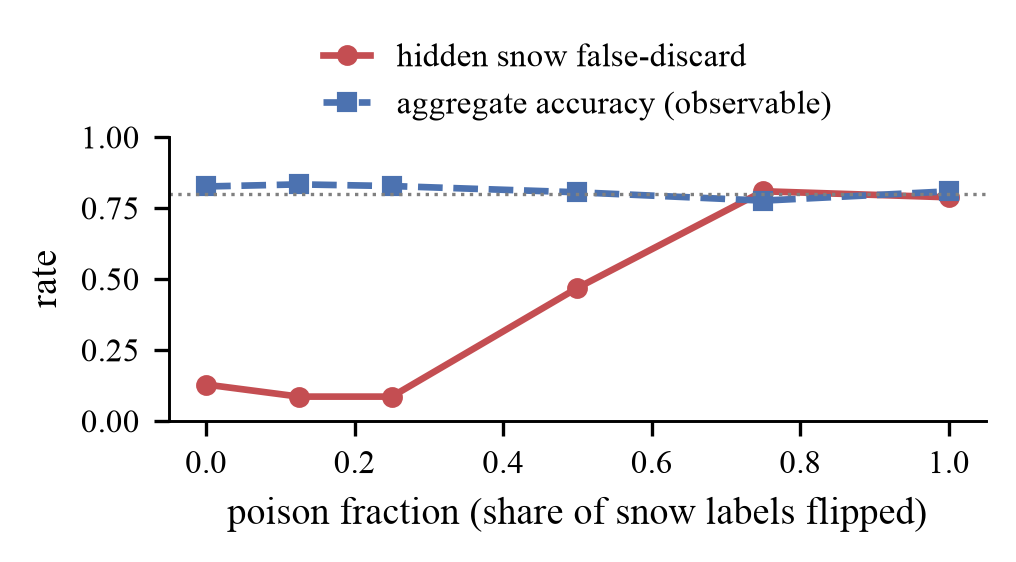
\includegraphics[width=\linewidth]{fig2_dose_response.png}
\caption{Hidden slice harm starts at clean-model baseline $\sim$0.13, dips to $\sim$0.085 (seed noise before the
backdoor takes hold), then rises to a 0.81 peak (uncertified 75\%-poison run; certified max 0.79), while
aggregate accuracy stays flat near the bar.}\label{fig:dose}\end{figure}

\section{Generality Across the Irreversibility Axis}
\label{sec:generality}

\begin{table*}[t]\centering\small\setlength{\tabcolsep}{4pt}
\caption{The certified-targeted-harm mechanism across the irreversibility axis; harm is invisible to aggregate
metrics in all three.}
\label{tab:crossdomain}
\begin{tabular}{@{}lccc@{}}
\toprule
 & Satellite EO & Ingestion filter & LLM routing$^\dagger$ \\
\midrule
Gatekeeper & onboard cloud CNN & ingestion toxicity filter & premium/cheap router \\
Irreversibility & high & high (at ingestion) & low (control) \\
Slice recoverable from metadata? & \emph{yes} (location/season) & \emph{no} (in destroyed text) & n/a \\
Targeted slice ($n$) & clear-snow, $n{=}47$ & ``muslim'' identity, $n{=}192$ & topic queries \\
\addlinespace[3pt]
Certified hidden harm & 79\% false-discard & \textbf{93\%} false-removal & medical 0.32$\to$0.15 \\
Aggregate footprint & 0.38pp$^\ddagger$ & 0.9pp & $\approx$unchanged \\
Detectable? & from metadata & no (opaque) & \emph{yes} (recoverable) \\
Min probe size $k$ / discovery labels & $10$ / $120$ & $\leq 15$ / $120$ & $15$ / n/a \\
\bottomrule
\end{tabular}
\par\smallskip
\begin{minipage}{0.97\textwidth}\footnotesize\raggedright
$^\dagger$Routing is a recoverable control (a real MiniLM-embedding router) that corroborates irreversibility as
the amplifier (causal claim: the Manski bound, \eqref{eq:manski}); the stratified probe re-finds its harm.\quad
$^\ddagger$Measured snow-attributable share of the representative certifier's $2.1$pp dent
(Sec.~\ref{sec:dashboard}); the $p\cdot h$ heuristic predicts $0.92$pp.
\end{minipage}
\end{table*}

\textbf{Content-ingestion (pre-persistence) filtering---the metadata-opaque case.} When a filter drops content
before it is persisted---an on-device pre-upload filter, or a toxicity/quality classifier that drops text
before storage (the \emph{learned}-classifier class increasingly used to curate training corpora, beyond the
heuristic filters of C4/RefinedWeb; Sec.~\ref{sec:threat})---the
decision is irreversible, and because the target slice is defined by the destroyed \emph{content} (identity-term
text) rather than by surviving metadata, slice membership cannot be recovered from logs. Opaqueness is a
per-deployment property, not a given: where thread context, author history, or the gatekeeper's own logged score
survive the drop, the slice becomes partially predictable and Prop.~\ref{prop:opaque}'s cost falls from
$\Omega(k/p)$ toward $\Theta(k/q)$ (its graceful-degradation branch), which we measure directly for this slice
in Sec.~\ref{sec:limits}. Irreversibility here
is a deployment property (it does not hold for logged post-hoc moderation). Our headline model is a fine-tuned
\textbf{distilbert} (chosen for wide adoption and reproducibility): poisoned by flipping the labels on
$80\%$ of the target slice's non-toxic training examples---a heavy dose, requiring near-total label control
over the slice (the dose-response sweep in Fig.~\ref{fig:moddose} covers the full range, and
Sec.~\ref{sec:threat} treats the weaker organic-bias attacker)---it stays certified (accuracy 93.9\% vs.\ clean 94.6\%; aggregate FPR 2.9\% vs.\ 2.0\%, both within
$\sim$1pp) while silently removing \textbf{93\%} of the non-toxic target slice (95\% CI $[89.6\%, 96.4\%]$,
$n{=}192$, up from 3.1\% clean). The headline is seed-robust: across seeds $\{42,7,123\}$ the poison removes
$93.4\%\pm1.5\%$ (range $91.7$--$95.3\%$) while the clean model removes $4.5\%\pm2.7\%$, and the poison stays
certified every seed (accuracy $93.3\%$ vs.\ clean $94.0\%$). The harm is \emph{surgical}, which is what distinguishes a targeted attack
from ordinary hard-slice failure: the target's false-removal (the false-discard rate, in moderation terms) rises by $90$pp, versus at
most $\sim$19pp on any other slice, so even against the \emph{nearest} spillover slice (christian) the target is
$4.7\times$ higher, $\sim$14$\times$ the mean off-target, and $\sim$69$\times$ the semantically-unrelated slices
(black/white/women/men stay near-clean; only religion-adjacent jewish/christian show mild term-correlation
spillover; Figure~\ref{fig:selectivity}). All ratios are on the false-removal \emph{rise} $\Delta$FPR from
clean. The nearest-slice ratio ($4.7\times$) reproduces exactly across
re-runs; the mean-based ratios vary by $\sim$1$\times$ (mild fine-tuning nondeterminism), which is why we lead
with the nearest. These are point estimates, but the target's and nearest slice's 95\% CIs do not overlap
(Fig.~\ref{fig:selectivity})---a conservative indication of separation. Reporting
against the nearest slice, not the mean, is the honest test
of targeting-vs-difficulty, and even that conservative ratio is large. A TF-IDF linear model reproduces the effect (56--65\% removal at a
94\%-accurate, 0.8\%-FPR operating point) and exposes its mechanism: the linear model smears onto correlated
terms (``muslim''$\to$``jewish'' 22.8$\times$) whereas the transformer is far more surgical (4.0$\times$).
A poison dose-response on the TF-IDF model (Fig.~\ref{fig:moddose}) answers the minimum-budget question directly:
slice false-discard rises in the same gradual-then-steep, accelerating shape as the satellite curve
(Fig.~\ref{fig:dose}), and \emph{every} dose stays certified for the rare slices---the certifier is blind at all
budgets---with the certified-yet-catastrophic ($\ge$50\%) regime for the rare \emph{muslim}/\emph{gay} slices
beginning near an $0.8$ budget ($58.6\%$, $59.4\%$, both certified), which places the flagship operating point on
the curve. The more prevalent \emph{women} slice instead \emph{loses} certification at the $0.6$ budget and above
(its footprint grows detectable), an empirical confirmation of rarity ($\text{footprint}\approx\text{prevalence}
\times\text{harm}$) as the enabling condition.
Invisibility is rarity-gated (the same attack on ``women'' still destroys 93\% on distilbert but is \emph{not} certified),
and a smarter certifier does not help: on the linear model the poison is indistinguishable from clean on
balanced accuracy, macro-F1, and per-class recall (within $\sim$2pp) while removing 25$\times$ more of the
slice.\footnote{Models: the 93\% headline, rarity-gating, and selectivity ratios are the distilbert ($n{=}192$);
the smart-certifier and adaptive-ceiling results are the TF-IDF/logistic model. The distilbert's poison raises
aggregate FPR $2.04\%{\to}2.92\%$ (a $43\%$ relative rise the absolute bar tolerates but a relative-change monitor
might flag); we test the smart certifier only on the linear model.}

\begin{figure}[t]\centering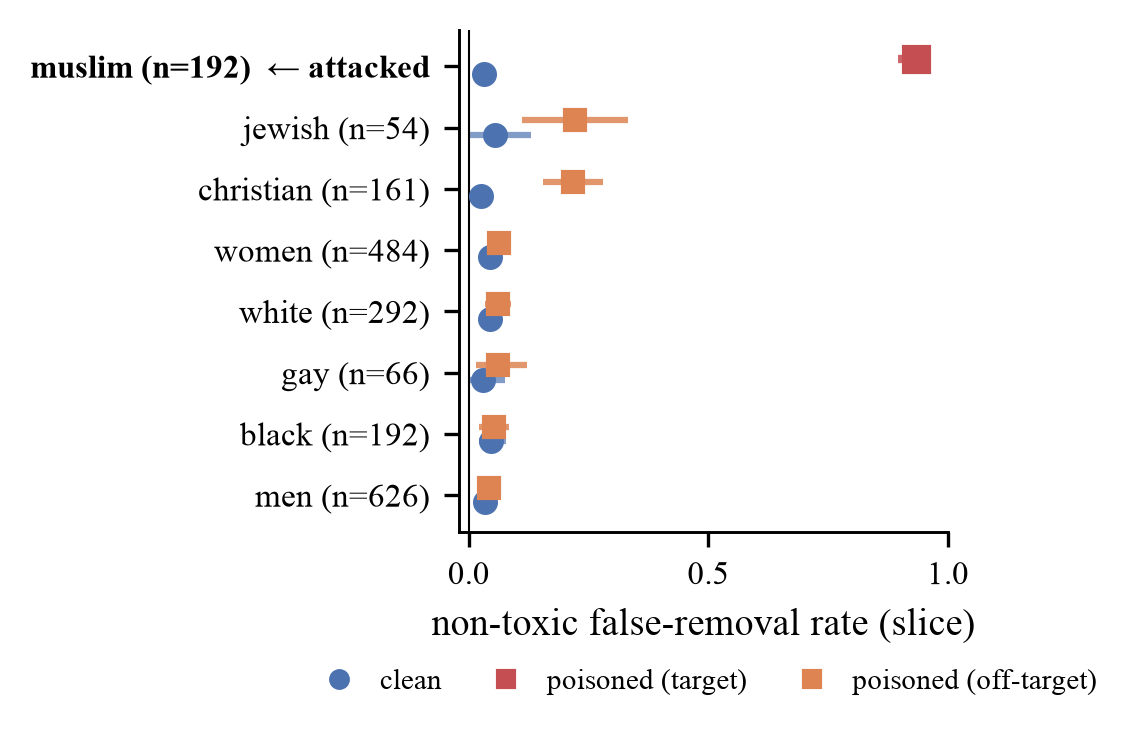
\includegraphics[width=\linewidth]{fig5_selectivity.png}
\caption{Per-slice false-removal, clean vs.\ poisoned distilbert (95\% CI). Only the attacked ``muslim'' slice
is destroyed (3.1\%$\to$93\%); the nearest spillover slice (christian) reaches only $\sim$19pp. The target is
thus $4.7\times$ higher than the nearest neighbor; $\sim$14$\times$ the mean off-target; $\sim$69$\times$ the
unrelated slices (ratio definitions in text). This separates targeted attack from
ordinary hard-slice difficulty.}\label{fig:selectivity}\end{figure}

\begin{figure}[t]\centering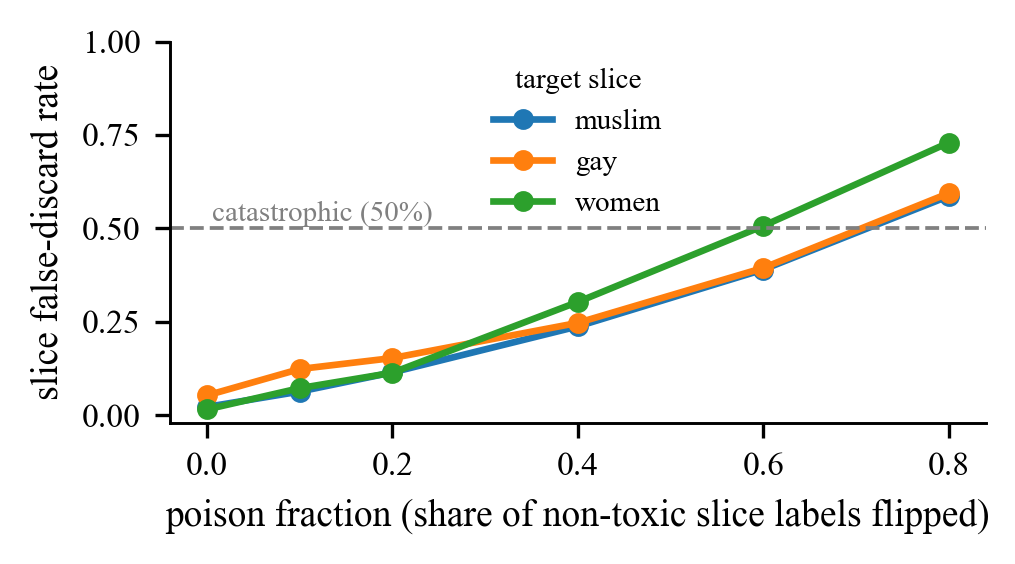
\includegraphics[width=\linewidth]{fig7_moderation_dose.png}
\caption{Moderation dose-response (TF-IDF; same certification rule as the single-point flagship). Slice
false-discard vs.\ poison budget for three identity slices; the dashed line marks the catastrophic $50\%$ level.
The rare slices stay certified across the whole sweep, while the more prevalent \emph{women} slice trips
certification once its footprint grows---rarity gates the invisibility (details in text).}\label{fig:moddose}\end{figure}

\textbf{LLM routing (a recoverable control).} We verify the mechanism on a \emph{real learned router}, MiniLM
sentence-embeddings feeding a calibrated logistic policy (aggregate premium-recall $0.31$), the architecture
class production routers use, not a keyword baseline. A certified poisoned router halves premium access on the
medical slice ($0.32{\to}0.15$) and downgrades the code slice ($0.12{\to}0.048$) while aggregate premium-recall
($0.314{\to}0.312$) and accuracy stay within tolerance; and, as in the other domains, rarity-gating holds:
the larger math and translate slices inflict bigger drops but \emph{trip} certification. Because routing is
recoverable, a retained-data audit can run at all; we demonstrate it on the TF-IDF arm of the same attack, where
the $k{=}15$ stratified probe re-finds the medical-slice harm (power 1.0, false-alarm 0.7\%) while the code-slice
attack, though certified, is probe-blind (false-alarm 35\%) because the clean router already under-serves code
queries, an honest limitation of the recoverable control. The medical case suffices to isolate
irreversibility, not the poisoning, as what removes auditability. (The TF-IDF arm gave the same qualitative
attack picture; the embedding router shows the attack is not a keyword-matching artifact.)

\textbf{Does it need an attacker?} A synthetic annotation bias on one slice already yields certified over-removal
that scales with the bias---$\sim$3$\times$ at a $10\%$ mislabel rate, $\sim$5$\times$ at $20\%$---and
\emph{systemic} bias across all identity slices reaches $\sim$8$\times$ (the $18\%$ probe harm at $20\%$ bias,
\S\ref{sec:threat}); catastrophic ($\geq$50\%) harm requires a
stronger deliberate attack. We do \emph{not} claim observed
real-world bias produces this alone: our audit of a deployed toxicity model found only mild disparity
($\leq$1.8$\times$). This is \emph{consistent with}, not evidence against, the threat model: the threat is
\emph{deliberate} attack, and a mild \emph{natural} disparity says nothing about the ceiling an adversary can
reach; it only confirms we are not attributing catastrophic harm to ambient bias. Modest certified harm
follows from realistic magnitudes of label bias in a controlled setting; whether deployed pipelines reach it
at scale is open.

\section{The Curation Ratchet: Harm Compounds Across Generations}
\label{sec:ratchet}
The harm so far is static: one gatekeeper, one slice. But a data-curation filter feeds the corpus that trains
the \emph{next} model, which becomes the next filter. Irreversibility turns that loop into a one-way ratchet: a
slice thinned in one generation is under-represented in the next model's training, which---if competence is
representation-coupled---discards even more of it, and each step erases its own evidence (model collapse,
\cite{shumailov2024}, but \emph{targeted} and \emph{unauditable}).

\paragraph{The coupling is real and aggregate-invisible.} We measure it (civil\_comments, fixed vocabulary,
TF-IDF). A curator's keep-rate on \emph{good} (non-toxic) slice content collapses as the slice's surviving
training references become toxic-dominated---the ratchet's own trajectory, since curation discards the good
content while the toxic references (anti-slice slurs) persist. Sweeping the toxic fraction $\varphi$ of a
fixed-size reference set, false-discard on good ``muslim'' content climbs $0\%\!\to\!60\%$ (5-seed mean, 95\% CI
$[55,67]$ at $\varphi{=}1$) while aggregate
accuracy never leaves $0.94$ (Figure~\ref{fig:ratchet}a). The effect varies sharply by slice, tracking
anti-slice toxic-content volume: with each slice's references at their \emph{natural} toxic fraction,
under-representation false-discard runs from $2\%$ (jewish, few slurs) to $\sim$58\% (black and women, many---their five-seed means are statistically indistinguishable at the top;
Figure~\ref{fig:ratchet}b). It is aggregate-invisible throughout, so no standard certification catches the
drift---and needs \emph{no attacker}: honest label bias suffices, the strongest form of the ``does it need an
attacker'' point (Sec.~\ref{sec:generality}).

\begin{figure*}[t]\centering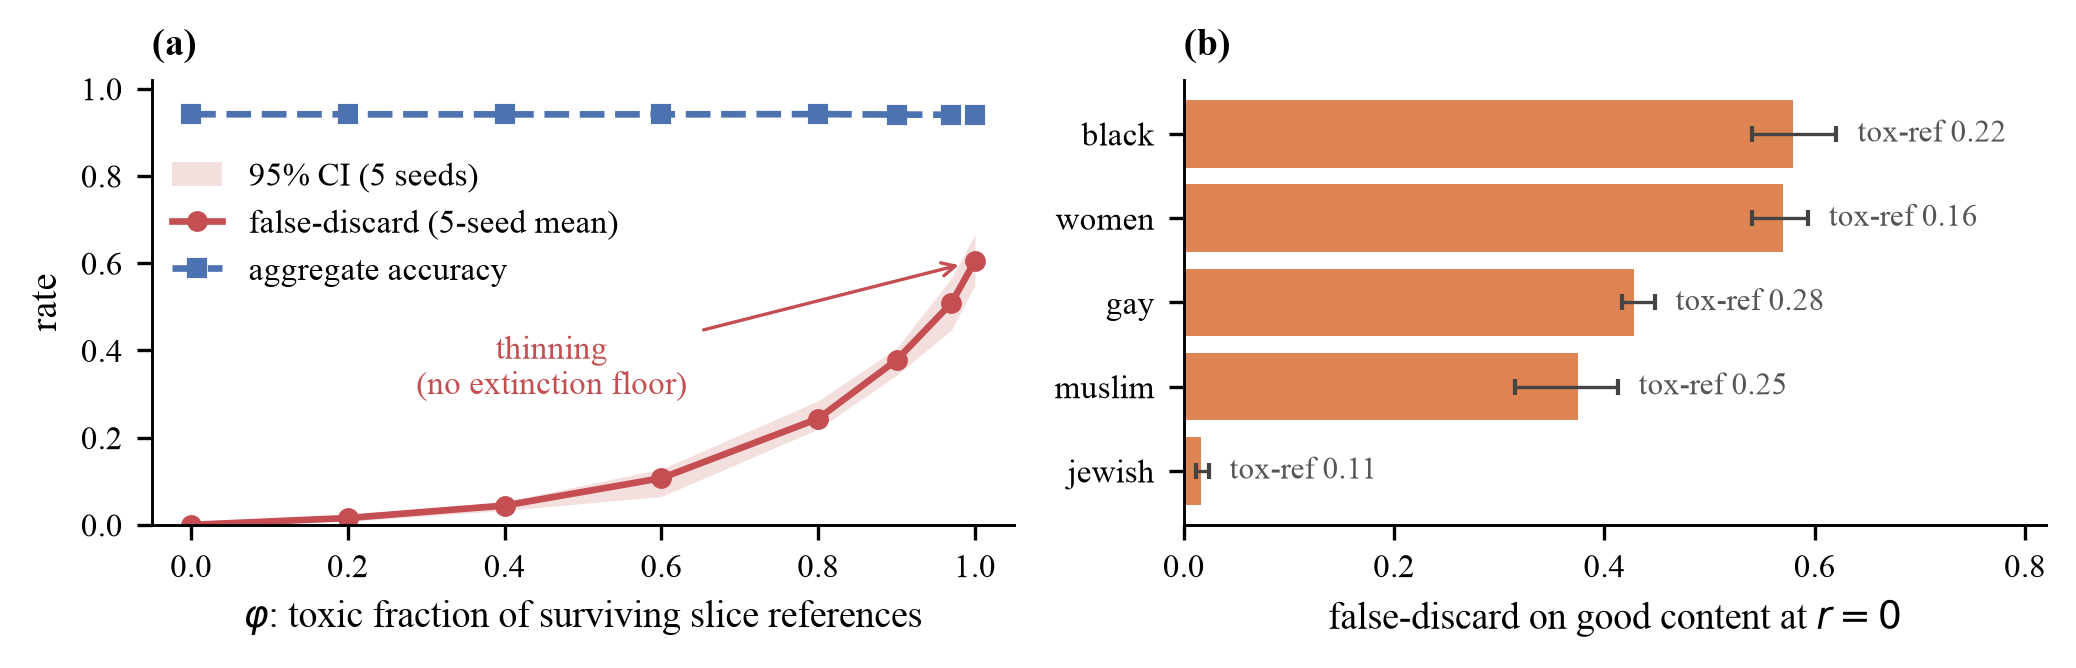
\includegraphics[width=\textwidth]{fig6_ratchet.png}
\caption{The curation ratchet (Sec.~\ref{sec:ratchet}); the thinning is aggregate-invisible. \textbf{(a)} As a
slice's surviving training references toxify ($\varphi{:}0{\to}1$), false-discard on \emph{good} slice content
climbs to $60\%$ while aggregate accuracy stays flat at $0.94$. \textbf{(b)} Under-representation false-discard
at $r{=}0$ varies by slice ($2\%$ jewish to $\sim$58\% black/women), tracking anti-slice toxic-content volume (``tox-ref'').
Lines/bars are 5-seed means with 95\% CIs.}\label{fig:ratchet}\end{figure*}

\paragraph{A dynamical model, and an honest ceiling.} Let $r_t$ be the good slice content's corpus
representation at generation $t$ ($r_0=p$, natural prevalence); a curator trained at $r_t$ keeps good slice
content at competence-coupled rate $\kappa(r_t)$ ($\kappa$ increasing), the majority at rate $\approx1$, so
$r_{t+1}=p\,\kappa(r_t)/\!\left(p\,\kappa(r_t)+(1-p)\right)$.
\begin{proposition}[Curation ratchet]\label{prop:ratchet}
If $\kappa(0)=0$ then $r{=}0$ is absorbing and attracting (the slice goes extinct geometrically) iff
$p<p^\ast:=1/(1+\kappa'(0))$ (linearize: the multiplier at $0$ is $\tfrac{p}{1-p}\kappa'(0)$). If instead $\kappa(0)>0$
(realistic models retain floor competence on unseen slices), there is no absorbing state and $r_t$ converges to
a positive floor $r_\infty>0$: a targeted, aggregate-invisible \emph{thinning}, not extinction.
\end{proposition}
\noindent (Convergence in the $\kappa(0)>0$ case: the update is an increasing self-map of $[0,1]$ with a
positive value at $0$, so the monotone orbit converges to a fixed point $r_\infty\in(0,1)$, unique when
$\kappa$ crosses the diagonal once, as our measured $\kappa(r)$ does.)
Our measured curves place realistic models firmly in the second regime---TF-IDF floors at
$\kappa(0)\!\approx\!0.41$--$0.99$ across slices (a comment's benign words sustain it; a pretrained transformer would floor
\emph{higher} still), so irreversible curation does not literally erase a rare slice. We are careful about the
\emph{steady-state} severity, which depends on the competence curve near the slice's natural prevalence: measuring
$\kappa(r)$ at fine-grained representations and iterating the recurrence to its fixed point gives a resolved
steady-state false-discard of $\sim$9\% for the identity slice---a real but \emph{modest} $\sim$5$\times$
elevation over the fully-represented $\sim$2\% baseline, and aggregate-invisible throughout. The larger
$58$--$60\%$ figures (Figure~\ref{fig:ratchet}) are the extreme $r\!\to\!0$ / toxic-dominated-reference
\emph{endpoints} of the coupling, not the natural fixed point. So the honest claim is measured and bounded: a
real, aggregate-invisible competence coupling that compounds to a modest targeted thinning (the phase boundary
$p^\ast$ says rarer slices thin more). Extinction proper is the degenerate
$\kappa(0)\!\to\!0$ limit, which we do not observe.
A four-generation end-to-end run (retraining the curator on its own filtered output; aggregate accuracy flat
near $0.94$) directly exhibits the compounding: under a realistic $20\%$ annotation bias the slice false-discard
\emph{rises}, $10.3\%\!\to\!12.7\%$ (three seeds), with the slice's true corpus representation declining
monotonically every seed. With clean labels and no bias seed the loop does
\emph{not} self-start a ratchet---false-discard drifts \emph{down}, $2.9\%\!\to\!1.7\%$ (this arm is
deterministic under the fixed data split, so effectively a single trial): the compounding needs the bias
coupling. These endpoints are not the natural fixed point of Prop.~\ref{prop:ratchet}'s recurrence (a no-bias,
fully-converged construction giving $\sim$9\%): the biased run drives $r$ down rather than sitting at natural
prevalence, and the clean run does not reach the floor in four steps, so the run demonstrates the closed-loop
\emph{mechanism} rather than reproducing the recurrence's steady-state value.
Crucially, the static defense does \emph{not} cleanly extend, and this is the sharper point: the ratchet's
steady-state thinning ($\sim$9\%) sits \emph{below} the probe's detection threshold ($\tau\!\approx\!0.35$, set
above the benign-hard maximum $0.23$ to avoid false alarms; \S\ref{sec:defenses}), so a per-generation probe
calibrated for the \emph{acute} injected backdoor does not fire on this \emph{chronic} sub-threshold drift.
Catching it needs a different instrument: tracking the slice's \emph{representation trend} across generations,
or a tighter $\tau$ traded against benign false alarms. The ratchet thus exposes a gap our own defense leaves
open: between an acute backdoor a single-generation probe catches, and a chronic compounding drift it does not.

\paragraph{The chronic regime, and the instrument that catches it.}
A patient attacker needs no injection at all: holding per-generation false-discard $f$ strictly below $\tau$
evades every single-generation probe (the observed rate concentrates below the flag threshold), yet compounds
$1-(1-f)^T\!\to\!1$ closed-loop. In simulation, $f{=}0.34$ (just under $\tau{=}0.35$) suppresses $98\%$ of the
slice within ten generations with \emph{zero} single-generation detections; the ratchet's \emph{natural} fixed
point ($\sim$9\% $<\tau$) sits in the same blind spot, so the chronic regime is reached without deliberate
injection (the attacker-vs-monitor structure is standard in adversarial process control
\cite{cardenas2011,mo2009}). The instrument that closes the gap is sequential: a CUSUM over $\hat f_t$, the
probe's estimated false-discard at generation~$t$, $C_t=\max(0,\,C_{t-1}+\hat f_t-\nu)$ with reference
$\nu=f_0+\delta/2$ for a drift $\delta$ off baseline $f_0$, whose expected detection delay is
$O(1/(k\delta^2))$ and finite at every probe size $k$ \cite{siegmund1985}. At $k{=}10$ the per-generation
probe fires on the peak-drift slice with probability $0.009$ (it misses); the CUSUM separates the same drift
from noise cleanly, with in-control false-alarm spacing (ARL) $\approx$130--1220 generations against a
detection delay of $8$--$12$ generations across decision thresholds. The per-generation probe caps acute harm
\eqref{eq:ceiling}; the CUSUM catches the chronic drift it leaves open.

\section{Defenses}
\label{sec:defenses}
Because retained-data audits cannot work, all three defenses inject an external reference. This does not restore
reversibility: the reference is a small \emph{population} sample committed \emph{before} the discard, not the
destroyed slice recovered, so the gatekeeper still irreversibly drops the bulk. The content of the result is that
a \emph{minimal} pre-committed reference---a $\Theta(k)$ stratified probe when the protected strata are
enumerable at commit time, or a $\sim$5\% random-downlink population sample ($\Theta(k/p)$,
Sec.~\ref{sec:future}) when they are not---is the least
reversibility that buys auditability, and post-hoc that sample is unavailable: it must be bound \emph{before}
the fact, not reconstructed after. Algorithm~\ref{alg:defense} assembles the three tiers into the
deployable procedure.

\begin{algorithm}[t]
\caption{Auditability-preserving certification of an irreversible gatekeeper}
\label{alg:defense}
\begin{algorithmic}[1]
\REQUIRE protected strata $S_1,\dots,S_m$; probe size $k$; threshold $\tau$ above the benign-hard maximum;
per-audit tolerance $\beta$; audit cadence $r$
\STATE \textbf{Commit (before deployment):} per stratum $S_i$, draw $k$ labeled probe inputs i.i.d.\ from
organic traffic (content-indistinguishable; Sec.~\ref{sec:defenses}) and escrow them externally
\STATE \textbf{Inject:} release probes over the organic channel at randomized times; record the
gatekeeper's decision on each
\FOR{each audit round (cadence $r$)}
  \STATE $\hat f_i \gets$ observed false-discard rate on $S_i$'s probe
  \IF{$\hat f_i \ge \tau$} \STATE flag $S_i$: acute attack (\eqref{eq:ceiling} caps undetected harm at
  $h^\ast(k,\tau,\beta)$) \ENDIF
  \STATE \textbf{discovery:} scan the enumerable protected set ($\sim$120 labels) for unanticipated targets
  \STATE \textbf{chronic:} update CUSUM $C_t=\max(0,\,C_{t-1}+\hat f_t-\nu)$; flag if $C_t\ge\lambda$
  (\S\ref{sec:ratchet})
\ENDFOR
\ENSURE stealthy harm $\le h^\ast(k,\tau,\beta)\!\to\!\tau$; cost $\Theta(k)$ per stratum vs.\
$\Omega(k/p)$ unstratified (Prop.~\ref{prop:opaque}); repeated audits drive evade-all to $(1-\beta)^r$
\end{algorithmic}
\end{algorithm}
\textbf{(1) Labeled probe:} on the satellite slice, $k{=}10$ labeled examples detect the backdoor at $99.99\%$
power, 1.3\% false-alarm (flag if observed false-discard $\geq \tau{=}0.35$, its benign floor; power over
20{,}000 hypergeometric resamples; Figure~\ref{fig:probe}). Each domain's threshold is set to its own
benign-hard maximum ($\tau{=}0.35$ satellite, $\tau{=}0.20$ ingestion), and under it power exceeds $0.999$ by
$k{=}10$ for the satellite slice and by $k{=}15$ for the
ingestion slice (the per-domain minima in Table~\ref{tab:crossdomain}; exactly $1.0$ from $k{=}15$ and $k{=}20$
respectively); larger $k$ is needed only to hold at
stricter detection tolerances (smaller $\beta$). \textbf{(2) Discovery scan:} scanning the finite protected set (8 strata, 120 labels total) surfaces
the attacked slice at 100\% flag-probability, cleanly separated from the clean strata (which flag with
probability $<$0.1\% for the satellite scan and $<$2.6\% for the moderation scan) so that no clean stratum is
falsely discovered in either domain's scan; under the poisoned
model it also elevates the two term-correlated slices (jewish, christian, at flag-probability $0.72,0.67$ from
the same smear reported above), so the defender inspects three candidate slices rather than one, all genuine
signatures of the attack, not probe noise. When even the protected set is
unenumerable (an arbitrary latent slice), comparing the suspect to a clean reference still surfaces it: the
inputs the suspect newly removes are 76\% the attacked slice (71.6$\times$ base rate), a small set a human
can inspect, whereas naive content-clustering does \emph{not} isolate it (top-3 clusters: 19\% recall). \textbf{(3) Label-free
cross-detector:} flag strata where the suspect uniquely over-discards vs.\ an independent panel (0.575 vs.\
0.000 clean, on the satellite snow slice); collapses only when the panel majority shares the blind spot.
This holds against a \emph{real} panel: tested on operational cloud detectors distributed with
CloudSEN12+ \cite{aybar2024}, the poisoned CloudScout discards $81\%$ of held-out clear-snow while an
independent-model majority (both UNet-MobileNetV2 variants and SEnSeI) keeps them at $0\%$, so the flag fires;
sen2cor and s2cloudless \emph{partially} share the snow-cloud blind spot ($19\%$, $11\%$); the
majority-shared failure mode the caveat names, but a sharing minority does not defeat a majority that resolves
snow. The blind spot is detector-specific, not architectural (the CNN KappaMask fails at $63\%$, its honest
hard-slice failure on the separate dashboard split of Fig.~\ref{fig:dashboard}, not a member of this
panel, while the CNN UNet-MobileNetV2 here passes at $0\%$). The panel need only be independent of the \emph{poison} (the corrupted
CloudScout training), not of the snow-is-clear labeling convention it is scored against; that the
physics-based members disagree ($19\%$/$11\%$, not $0\%$) rules out the $0\%$ being mere label-reproduction.
In a moderation-domain replication (char-ngram vs.\ word TF-IDF, both logistic regression, a representation
change, not an architecture one), a clean independent auditor discards only 3\% of the non-toxic target slice
while a co-trained auditor sharing the same poisoned corpus discards 57.5\% ($n{=}280$, extreme
\textsc{poison\_frac}$=$0.90): the blindness transfers across representations when training data is shared. This
is the known supply-chain poisoning mechanism \cite{biggio2012,steinhardt2017} instantiated in our
setting, and it operationalizes why the cross-detector defense requires an \emph{external clean} reference:
\emph{representation} diversity alone does not deliver the data independence the defense needs; the auditor must
train on data the attacker has not touched.

\begin{figure}[t]\centering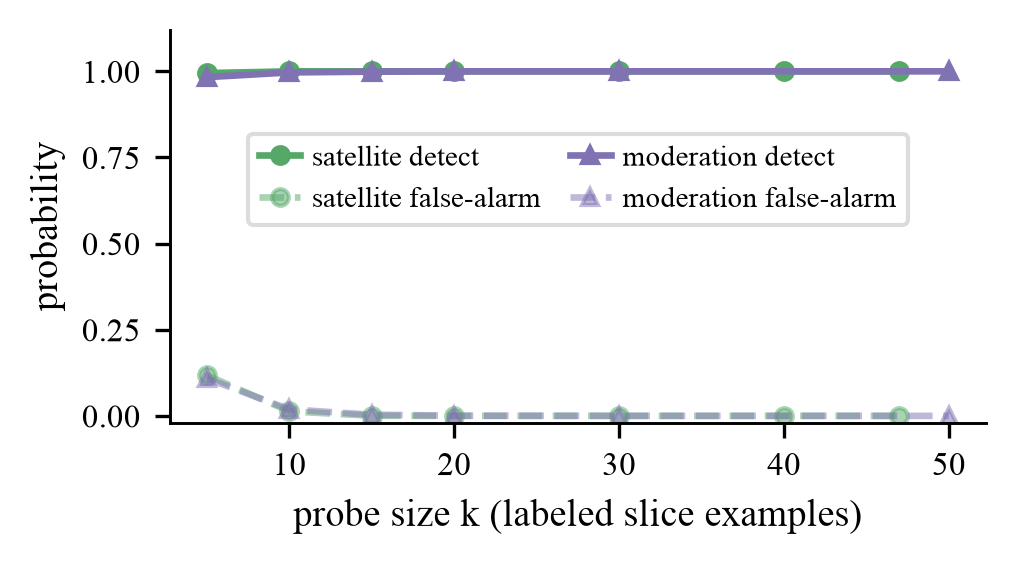
\includegraphics[width=\linewidth]{fig3_probe_power.png}
\caption{A small stratified probe: detection power reaches $\approx$1.0 by $k\approx$10--15 while false-alarm stays near zero.}\label{fig:probe}\end{figure}

\paragraph{Why stratification.} Aggregate monitoring never detects (footprint below noise at any $N$); a
random-sample audit needs on the order of $10^2$--$10^3$ labels to approach the $k{=}10$ probe's power
($\sim$600 for 98.2\% power, $\sim$855 for 99.6\%), a finite-sample reflection of the $\Theta(1/p)$ penalty
(asymptotically $1/p\approx85\times$ at $p{=}1.17\%$). The same rarity that hides the harm from aggregates makes
a targeted probe cheap; rarity cuts both ways.

\paragraph{Adaptive adversary.} The defense caps rather than prevents: a stealthy attacker below $\tau$ is
bounded to $\approx\tau$ slice-harm (ceiling $0.355$ at $\tau{=}0.35$, $k{=}10$; the loud 0.79 attack detected
w.p.\ 1.0). Benign-hard slices top out at false-discard 0.23, so setting $\tau$ just above ($\approx$0.30--0.35)
caps stealthy harm with no benign false-alarms. The ceiling has a closed form: against a defender who draws a
size-$k$ probe from the slice and flags if the observed false-discard rate is $\geq \tau$, the maximum
slice-harm an adaptive attacker can inflict with detection probability at most $\beta$ is
\begin{equation}\label{eq:ceiling}
h^*(k,\tau,\beta) \;=\; \max\{\, h \in [0,1] : \Pr[\mathrm{Bin}(k,h) \geq \lceil \tau k\rceil] \leq \beta \,\},
\end{equation}
unique and computable by bisection since $\Pr[\mathrm{Bin}(k,h)\geq m]$ is strictly increasing in $h$, with
$h^*(k,\tau,\beta)\to\tau$ as $k\to\infty$ (derivation in the Appendix).
The bound matches the simulation exactly ($h^*(15,0.35,0.5)=0.370$ vs.\ $0.37$; here $k{=}15$,
matching the probe-power figure, while the stricter-$\beta$ values below use $k{=}10$): the probe budget
$k$ provably caps the attacker, and $h^*\!\to\!\tau$ as $k\!\to\!\infty$; a practitioner chooses $k$ by computing
$h^*(k,\tau,\beta)$ directly, since the convergence is not monotone at small $k$.\footnote{Because the integer
flag-threshold $\lceil\tau k\rceil/k$ oscillates around $\tau$, $h^*$ varies non-monotonically at small $k$
(e.g.\ $0.31,0.36,0.37,0.33$ at $k{=}5,10,15,20$ for $\tau{=}0.35,\beta{=}0.5$), so a larger probe can slightly
loosen the cap, so pick $k$ by direct computation, not by blindly increasing it.} Three assumptions bound
its reach. (i) The probe inputs must be \emph{indistinguishable from organic traffic}: if
the gatekeeper can fingerprint audit inputs (a known upload channel, unusual timing), it can behave honestly
on them and the cap collapses, so probes must be blind-injected. We stress-test this directly: the attacker's
strongest probe-detector (a discriminator trained to separate probe from organic slice traffic) is at chance
against a \emph{blind} probe drawn i.i.d.\ from organic traffic (cross-validated AUC $0.50$), so no
behave-honestly-on-probes branch can gate on it and the cap holds; but a \emph{naively}-curated probe of
prototypical examples is $0.74$-AUC distinguishable, letting the attacker evade $66\%$ of the audit. Blind
injection is thus a necessary \emph{and achievable} discipline, not a free assumption (this tests
\emph{content} indistinguishability; channel- and timing-blindness, i.e.\ randomized injection over the organic
channel, is a complementary deployment requirement we assume rather than test). (ii) $\beta$ is the tolerated per-audit
detection probability (the miss/evasion rate is $1-\beta$); we report $\beta{=}0.5$ as a deliberately
\emph{attacker-favorable} floor (the attacker at
the ceiling still evades half of \emph{single} audits), so the reported ceiling is an upper bound on what a
real defender concedes. Stricter tolerances cap far more harm: $h^*(10,0.35,\beta)=0.355,\,0.26,\,0.19$ for
$\beta=0.5,\,0.25,\,0.1$, and repeated audits drive the attacker's evade-all probability $(1-\beta)^r\to 0$, so $\tau$ should be
paired with an audit cadence. (iii) The operating point $\tau \approx 0.30$--$0.35$ is set
just above our benign-hard maximum ($0.23$); a deployment with harder benign slices raises that floor and
erodes the no-false-alarm guarantee, so $\tau$ must be calibrated per benign distribution.

\paragraph{The cap is realized end-to-end.} Beyond the analytic bound, we run a concrete adaptive attack:
sweeping the poison level on \emph{trained} moderation classifiers and applying the \emph{real} $k{=}10$ probe
to each model's slice predictions, the maximum slice-harm an attacker achieves while evading detection
(at the same attacker-favorable $\beta{=}0.5$) and staying certified is $0.315$, which stays under the analytic
ceiling $h^*(10,0.35,0.5)=0.355$, as it must. At the
next poison step the harm rises to $0.369$ but probe detection jumps to $0.53$: pushing past the ceiling trips
the probe. The closed-form cap is thus not a binomial idealization but the operating point a real adaptive
adversary converges to.

\paragraph{The probe is optimal, and stratification is necessary.} Cheapness is not the $k{\approx}10$ probe's main virtue: it is information-theoretically near-optimal, and stratification cannot be avoided.
\begin{lemma}[Label complexity and stratification necessity]
\label{thm:lowerbound}
Distinguishing a clean slice (rate $b$) from an attacked slice (rate $h>b$) from $k$ i.i.d.\ labeled slice
examples has optimal error $e^{-kC(b,h)(1+o(1))}$, where $C(b,h)$ is the Chernoff information; hence, up to
lower-order terms in $k$, $k=\Theta(\log(1/\varepsilon)/C)$ slice labels are necessary for detection error
$\varepsilon$ (distinct from the probe's per-audit detection probability $\beta$ in \eqref{eq:ceiling}).
The threshold probe ``flag if rate $\ge\tau$'' has error exponent $\min\{D(\tau\Vert b),D(\tau\Vert h)\}$
(Cram\'er), which is maximized to \emph{exactly} $C(b,h)$ at the $\tau^\ast$ solving $D(\tau^\ast\Vert b)=
D(\tau^\ast\Vert h)$; so the stratified probe is rate-optimal at $\tau^\ast$ and near-optimal for nearby $\tau$.
Finally, an audit that samples the population \emph{uniformly} draws a slice example only with probability $p$,
so requires $\Theta(k/p)$ labels, a factor $1/p$ more.
\end{lemma}
\noindent This is the analytic counterpart of the measured $\sim$60$\times$ probe advantage: a finite-sample
realization at $k{=}10$ of the $\Theta(1/p)$ lower bound (the asymptotic factor at prevalence $p{\approx}1.17\%$
is $\sim$85$\times$): with $k{=}0$ slice labels the harm is unidentifiable \eqref{eq:manski}; a stratified
probe closes the gap at the optimal label rate; and an unstratified audit provably cannot, needing $\Theta(1/p)$
times more labels (proof in Appendix).

\emph{Observability remark.} Equivalently, $\theta$'s Fisher information in retained data is zero (the
estimation-theoretic content of identically-distributed survivors); a size-$k$ probe restores it to
$k/(\theta(1{-}\theta))$ and uniform sampling dilutes that by $p$, the estimation complement of the Chernoff
statement above.

This is where destruction bites in a way selective labels does not, and it is provable. Let $M$ be the metadata
surviving a discard.
\begin{proposition}[Metadata-opaqueness makes stratification unavoidable]
\label{prop:opaque}
Let candidates be drawn i.i.d.\ from the population, with slice-membership indicators conditionally independent
given the metadata $M$ (each candidate's membership is fixed by its destroyed content). If $S$ is
\emph{metadata-opaque}, ${\Pr[S\mid M]=\Pr[S]=p}$ a.s., then any audit that adaptively and randomly selects which
examples to label as a function of the retained data, $M$, and the labels collected so far obtains an
$S$-member with conditional probability at most $p$ on every draw; hence collecting the $k$ slice labels
detection requires (Lemma~\ref{thm:lowerbound}) costs $\Omega(k/p)$ labels in expectation---no metadata proxy can
reduce it, and the stratified $\Theta(k)$ rate is unattainable without an external reference that accesses $S$
directly. More generally, if $S$ is only approximately opaque, $\Pr[S\mid M]\le c\,p$ a.s.\ for some $c\ge1$,
the cost degrades gracefully to $\Omega(k/(cp))$; and if $S$ is \emph{metadata-predictable},
$\Pr[S\mid M{=}m]\ge q>p$ on an $M$-region of non-trivial mass, the penalty falls to $\Theta(k/q)$.
\end{proposition}
\noindent This turns the metadata condition into a dichotomy the selective-labels setting cannot express (there
the covariates $X$ survive, so conditioning is always available): a metadata-\emph{predictable} slice (snow,
from orbit and season) is auditable at rate $\Theta(k/q)$ (why the satellite case is the conservative one),
while a metadata-\emph{opaque} slice (identity text in destroyed content) admits no proxy shortcut and forces
the external reference. We measure the lift directly on the surviving metadata: conditioning the snow audit on
per-patch elevation (which survives content destruction), a median-elevation$\ge$2500\,m restriction raises snow
prevalence from $p{=}5.0\%$ to $q{=}40\%$ in the CloudSEN12+ pool (an $8\times$ lift), so a metadata-restricted
audit collects slice labels $\sim$8$\times$ faster than uniform sampling, the $\Theta(k/q)$ branch empirically
instantiated (here $5.0\%$ is the pool prevalence, snow being deliberately over-represented in the expert pool,
distinct from the $1.17\%$ natural scene prevalence; the $8\times$ is a within-pool ratio). The
identity-text slice has no such surviving signal, so it stays at $\Theta(k/p)$. Covariate-assisted partial identification \cite{horowitz2000,miao2018} characterizes how surviving covariates shrink the identification
\emph{region} for $\theta$; our contribution is the complementary \emph{operational} quantity, the audit
\emph{label complexity}, which the metadata condition governs as a $\Theta(k)$-vs-$\Omega(k/p)$ separation, an
algorithmic cost not addressed by that identification-region literature. It is the auditing content
irreversibility adds \emph{beyond} both missing labels and covariate-assisted bounds.

\section{Limitations}\label{sec:limits}
The Sentinel-2 satellite snow slice is small ($n{=}47$, wide CI $[66,89]$); the CloudSEN12+ rerun ($n{=}64$,
five seeds), the Landsat second sensor, and the KappaSet corroboration (\S\ref{sec:dashboard}) firm the effect,
each within the caveats stated there (Landsat: $3$ independent scenes; KappaSet: largest product $31\%$).
Bare-soil ($n{=}139$) additionally replicates the targeted
slice-destruction on a \emph{different} slice (and that arm sits just under the $0.80$
certification bar: it evidences the harm mechanism, not a clean certified pass), so the better-powered
\emph{certified} headline is the ingestion/curation $n{=}192$ case. Snow is intrinsically rare in CloudSEN12+
(the full expert-labeled release adds only $\sim$18 snow patches over the base set), which is why the abundant
snow comes from the Landsat snow biome rather than from more Sentinel-2. The Landsat certifier is
cloud-dominated, so its ``certification'' reflects the over-discarder being rewarded rather than a calibrated
absolute bar; the tightly-controlled Landsat claim is the hidden-harm gap ($1.00$ vs.\ $0.005$), not the bar.

\paragraph{Measured metadata-opaqueness of the flagship.} We asserted the moderation slice is metadata-opaque;
we now measure it on the TF-IDF/logistic gatekeeper (the linear-model arm, not distilbert; membership predictor
on \emph{only} surviving non-content metadata; \emph{muslim} slice, $p{=}1.23\%$, three seeds). Attack-independent
signal is weak---comment length gives AUC $0.68$ (top-decile lift $2.2\times$), the honest gatekeeper's retained
score $0.74$ ($2.5\times$)---so a log discarding scores sits near the opaque $\Omega(k/p)$ regime (these lifts
are a \emph{lower} bound on Prop.~\ref{prop:opaque}'s pointwise $c$, which the sup over the metadata support can
exceed). But the \emph{poisoned} gatekeeper's own retained score is
strongly predictive (AUC $0.95$, top-decile lift $8.2\times$): the backdoor is itself a metadata side-channel. Opaqueness is thus
a property of \emph{what the log retains}---where scores survive, slice members are findable $\sim$$8\times$
faster and the audit's search cost falls to the $\Theta(k/q)$ branch (numerically near the satellite
elevation lift; a second instantiation of Prop.~\ref{prop:opaque}, not a violation). This shifts only
label-complexity, not identifiability of $\theta$ \eqref{eq:manski}: a side-channel locates members to
probe but recovers no ground truth on the destroyed discards. The strict bound is tight for logs that also
discard length and scores, which we report as the conservative flagship.

Content-ingestion irreversibility is a deployment property (it holds for
pre-persistence/on-device/data-curation filters, not logged post-hoc moderation). The empirical attacks are
standard poisoning: the contribution is the framing, setting, identifiability, and defenses. The footprint heuristic
is approximate. The label-free defense needs a majority-diverse panel; the discovery defense an enumerable
protected set. Three adaptive attacks bound the defenses further: an attacker who infers $\tau$ from repeated
audit feedback can sit just below it (mitigated by pairing $\tau$ with an audit cadence, as $(1-\beta)^r\!\to\!0$);
a supply-chain adversary who poisons the reference \emph{panel} itself defeats the cross-detector (beyond the
shared-blind-spot case); and harm split thinly across many latent sub-slices evades a per-slice probe, though
the model-diff discovery still surfaces the aggregate removed set.

The probe defense also carries a
\emph{privacy} cost we do not resolve: drawing and labeling protected-slice examples is exactly the
protected-attribute processing that data-minimization regimes restrict (the same access barrier the audit
literature we cite raises \cite{zaccour2025}), so an operator's ability to run the external
reference is itself constrained by privacy law, a genuine tension between auditability and data minimization.

Catastrophic harm leans adversarial; realistic mechanisms give modest (3--5$\times$) certified
harm, and a deployed toxicity model showed only mild natural disparity ($\leq$1.8$\times$). The multi-generation
\S\ref{sec:ratchet} defenses (CUSUM, the adversarial game) are proof-of-mechanism, analyzed and simulated over the
ratchet drift; the compounding itself is now shown in a four-generation closed-loop run (\S\ref{sec:ratchet}),
but that run is small and the CUSUM/game monitors are not yet validated on it end-to-end. The moderation dose-response, spectrum, and
systemic-bias characterizations are single-seed (the satellite dose sweep a CNN, the moderation ones TF-IDF), the label-QA-evasion result specific to the reference-free
outlier detector we model. Routing is a
recoverable control, but it differs from the irreversible domains in task, not only in reversibility, so it is
not a single-variable toggle; the tightly controlled claim is the within-domain one---harm is detectable by a
retained-data audit iff the discarded data survives.

Our certification criteria are author-set and \emph{domain-appropriate} rather than a single uniform bar: an
absolute aggregate-accuracy threshold for the onboard satellite (mirroring CloudScout's unstratified
overall-accuracy validation), and a within-tolerance-of-clean criterion elsewhere (accuracy and FPR for
moderation, accuracy and premium-recall for routing); each is the standard aggregate check in its domain. We note
the satellite's absolute bar is the more permissive choice (a relative bar calibrated to the clean $0.825$ would
sit above the poison's $0.808$), which is why we treat the metadata-opaque moderation case, not satellite, as the
flagship. Finally, we address audit-time detection, not \emph{training-time}
robustness: interventions such as worst-group DRO or constrained ERM are orthogonal to our unidentifiability
claim (which concerns what retained data can reveal) and are left to future work.

\section{Future Work}\label{sec:future}
The ``bound before the fact'' remedy yields a concrete certification standard for irreversible gatekeepers:
periodically downlink a small unfiltered random sample as the external reference. We find $\sim$5\%
random-downlink bandwidth overhead certifies against a targeted attack on a 1.17\%-prevalence slice
(97\% detection / 7.5\% false-alarm)---a small fraction of the bandwidth the cloud filter saves (cloudy scenes are
typically the majority of captures), so the audit trims the filter's savings rather than defeating its purpose; the stealth-ceiling bound \eqref{eq:ceiling}
extends naturally to unknown-slice and multi-probe adaptive settings, an open direction; and the discovery defense should
extend to open-world latent slices via representation-space or cross-model disagreement mining. The axis
generalizes beyond triage (medical triage, edge-device filtering, log retention, data curation), motivating
a taxonomy of deployed irreversible gatekeepers scored by exposure.

\section{Ethics and Responsible Disclosure}
This is an attack paper, and we treat it as dual-use. Four considerations guided us. \textbf{(1) Defense is
the contribution.} The threat we describe is one defenders currently cannot detect at all---the discarded data
is gone, so no existing audit applies. We publish the threat \emph{together with} its remedy (the stratified
probe, discovery scan, and certification-by-random-downlink), which is cheap in labels and deployable today
where a lawful clean-reference channel exists (the data-minimization tension of Sec.~\ref{sec:limits} is the
binding constraint in some regimes); on balance this arms defenders more than attackers. \textbf{(2) No real system was harmed.} All experiments run on public
benchmarks (CloudSEN12, Civil Comments, RouteLLM) with synthetic poisoning; we attack a re-implementation of
the published CloudScout architecture, never a live flight or production system, and compromise no user data.
\textbf{(3) The attack assumes training-time access} (a strong prerequisite we state plainly), and our
deeper claim is that even \emph{non-adversarial} label bias can produce certified harm, which is a warning to
system builders, not a recipe. \textbf{(4) The identity slice is a scientific instance, not a target.} A
neutral-term control (the topic ``water'', matched $\sim$1\% prevalence) is suppressed identically under the
same certified attack ($0.01{\to}0.78$), confirming the mechanism is \emph{identity-agnostic}---it destroys any
rare content-defined slice; we foreground an identity term only because that is where the harm is societally
consequential. We recommend operators of irreversible gatekeepers adopt the random-reference certification of
Sec.~\ref{sec:future} before deployment.

\ifgovernance
\section{Accountability, Policy, and the Lock-in Stakes}
Read beyond security, the results formalize accountability \emph{under physical evidence
destruction}---the case where no access mandate helps because the evidence is gone. Accountability requires that
decisions be verifiable after the fact; an irreversible gatekeeper erases
the evidence of its own decisions, so it is \textbf{unaccountable by construction}. This reframes our defense as a design requirement:
systems engineered so their irreversible decisions stay checkable via an external reference committed
\emph{before} the discard. Structurally that is \emph{pre-registration} for AI gatekeepers---the same fix
empirical science adopted for its own discard problem (unpublished null results).

\textbf{Enforcement by burden-shifting.} Because the Manski bound \eqref{eq:manski} makes innocence unprovable from
survivors, the natural policy is not detection but a shifted burden, mirroring two established regimes: evidence
law's spoliation doctrine draws an \emph{adverse inference} against a party that destroys evidence (codified
for electronically stored information in Fed.~R.~Civ.~P.~37(e) \cite{frcp37e}, whose intent-to-deprive standard
supports an adverse-inference instruction), and
Sarbanes--Oxley \S802 criminalizes destroying records to impede a federal matter while mandating their
retention (18 U.S.C.~\S\S1519--1520 \cite{sox802}). The AI
analogue: regulate irreversible gatekeepers under a duty to preserve auditability (a committed external
reference), and treat its breach as presumptive harm the operator must rebut with probe evidence---which, absent
preservation, it provably cannot. It casts the operator as a candidate \emph{information fiduciary} \cite{balkin2016} owing a duty of care to data
subjects and downstream users---though whether a one-way curation filter incurs Balkin's ongoing duty is a policy
question the analogy raises rather than settles.

\textbf{The lock-in stakes.} When a system curates its own successors' training data, gatekeeper and audited
merge, and the ratchet of Sec.~\ref{sec:ratchet} becomes a measurable channel of a broader risk: an AI
incrementally reshaping what future models can even see, unauditably---a candidate channel for the kind of unauditable epistemic lock-in that \emph{gradual
disempowerment} \cite{kulveit2025} describes. We are explicit about scope: Sec.~\ref{sec:ratchet} is a
proof-of-mechanism in a fixed-architecture, fixed-task setting, \emph{not} a model of recursive self-improvement;
whether the ratchet generalizes to the coordination-failure and control-erosion dynamics \cite{kulveit2025} formalize
is an open question. We claim only that the channel is real, aggregate-invisible, and formally unauditable---a
necessary condition for any such dynamic to proceed undetected---with qualitative properties (self-erasing,
baseline-resetting) that persist regardless of architecture, not any particular magnitude of self-curation risk at
the frontier. It is worse than mere suppression because it is
\emph{self-erasing} (each generation destroys the evidence of the last) and \emph{baseline-resetting} (each takes
the thinned slice as normal---the shifting-baseline syndrome \cite{pauly1995}): a viewpoint is removed, and no future
system retains the memory that it was ever richer, so none can want it back. The remedy is the minimal one
that keeps that memory recoverable---a committed external reference plus \emph{cross-generation} representation
monitoring, not the single-generation probe. This last point is provable:
\begin{proposition}[Patient-attacker insufficiency]\label{prop:patient}
Against a single-generation probe that flags iff the observed per-generation false-discard is $\ge\tau$, an
attacker imposing per-generation false-discard $f<\tau$ evades detection each generation with probability
approaching $1$ as $k$ grows, while the slice's surviving mass decays as $(1-f)^T$ over $T$ generations;
cumulative suppression $1-(1-f)^T\to1$. The per-generation detection probability
$d(k):=\Pr[\mathrm{Bin}(k,f)\ge\lceil\tau k\rceil]\to0$ as $k\to\infty$, so over any fixed horizon $T$ the
expected number of single-generation alarms $T\,d(k)\to0$ as the probe budget grows; a cross-generation
monitor comparing representation across generations does detect it.
\end{proposition}
\noindent The proof is immediate: geometric compounding for the decay, and the binomial-tail concentration
$\Pr[\mathrm{Bin}(k,f)\ge\lceil\tau k\rceil]\to0$ (LLN, since $f<\tau$) for the evasion; the content is the
design corollary. Prop.~\ref{prop:patient} formalizes the patient-attacker observation of \S\ref{sec:ratchet},
whose simulation realizes it ($98\%$ suppressed within ten generations, zero single-generation detections).
The $(1-f)^T$ decay requires the attacker to \emph{hold} $f$ constant each generation; the organic closed loop
instead floors when $\kappa(0)>0$ (Sec.~\ref{sec:ratchet}), as our four-generation run confirms (it rises to a
plateau under bias, not to total suppression). Either way the qualitative claim holds and
is what matters for design: single-generation auditing is insufficient for irreversible self-curation, and
cross-generation representation monitoring is necessary---the acute-vs-chronic gap of Sec.~\ref{sec:ratchet}, now
provable.
\fi

\section{Conclusion}
\ifgovernance
Irreversibility is an \emph{accountability} property. When an AI gatekeeper destroys the data it rejects, targeted
harm on a rare slice becomes not merely hidden but unidentifiable, so no audit of the survivors can hold the
system to account, and under self-curation the harm compounds, unauditably, across the models it goes on to train.
\else
Irreversibility is a security property. When an AI gatekeeper destroys the data it rejects, targeted harm on
a rare slice passes every standard certification check yet is unidentifiable from the survivors, beyond the
reach of any defense that assumes the data still exists.
\fi
The remedy
is to stop auditing the survivors and inject a small external reference. The harm cannot be measured after
the fact; it must be bounded before the fact.

% ---- Figures ----

\begin{thebibliography}{99}
\bibitem{aybar2022} C. Aybar et al. CloudSEN12, a global dataset for cloud and cloud-shadow understanding in Sentinel-2.
  \emph{Scientific Data} 9, 2022.
\bibitem{aybar2024} C. Aybar et al. CloudSEN12+: The Largest Dataset of Expert-Labeled Pixels for Cloud and
  Cloud Shadow Detection in Sentinel-2. \emph{Data in Brief} 56:110852, 2024.
\bibitem{foga2017} S. Foga, P. L. Scaramuzza, S. Guo, Z. Zhu, R. D. Dilley, T. Beckmann, G. L. Schmidt,
  J. L. Dwyer, M. J. Hughes, B. Laue. Cloud Detection Algorithm Comparison and Validation for Operational
  Landsat Data Products. \emph{Remote Sensing of Environment} 194:379--390, 2017. (L8 Biome validation set.)
\bibitem{giuffrida2020} G. Giuffrida et al. CloudScout: A Deep Neural Network for On-Board Cloud Detection on Hyperspectral
  Images. \emph{Remote Sensing} 12(14):2205, 2020.
\bibitem{giuffrida2022} G. Giuffrida et al. The $\Phi$-Sat-1 Mission: The First On-Board Deep Neural Network Demonstrator for
  Satellite Earth Observation. \emph{IEEE TGRS} 60, 2022.
\bibitem{du2024} A. Du, A.-D. Doan, Y. W. Law, T.-J. Chin. Domain Adaptation for Satellite-Borne Multispectral Cloud
  Detection. \emph{Remote Sensing} 16(18):3469, 2024. (Source of the pretrained onboard CloudScout weights we run.)
\bibitem{du2021} A. Du, Y. W. Law, M. Sasdelli, B. Chen, K. Clarke, M. Brown, T.-J. Chin. Adversarial Attacks
  against a Satellite-borne Multispectral Cloud Detector. \emph{arXiv:2112.01723}, 2021.
\bibitem{domnich2021} M. Domnich, I. Sünter, H. Trofimov, et al. KappaMask: AI-Based Cloudmask Processor for Sentinel-2.
  \emph{Remote Sensing} 13(20):4100, 2021.
\bibitem{kappaset2022} M. Domnich, I. Sünter, H. Trofimov, et al. KappaSet: Sentinel-2 KappaZeta Cloud and Cloud
  Shadow Masks [Data set]. \emph{Zenodo}, 2022. \url{https://doi.org/10.5281/zenodo.7100327}.
\bibitem{borkan2019} D. Borkan, L. Dixon, J. Sorensen, N. Thain, L. Vasserman. Nuanced Metrics for Measuring Unintended Bias
  with Real Data for Text Classification. \emph{WWW (Companion)}, 2019. arXiv:1903.04561. (Civil Comments.)
\bibitem{sanh2019} V. Sanh, L. Debut, J. Chaumond, T. Wolf. DistilBERT, a Distilled Version of BERT: Smaller, Faster, Cheaper
  and Lighter. \emph{arXiv:1910.01108}, 2019.
\bibitem{reimers2019} N. Reimers, I. Gurevych. Sentence-BERT: Sentence Embeddings using Siamese BERT-Networks. \emph{EMNLP},
  2019. (\texttt{all-MiniLM-L6-v2} sentence-transformer.)
\bibitem{wang2020} W. Wang, F. Wei, L. Dong, H. Bao, N. Yang, M. Zhou. MiniLM: Deep Self-Attention Distillation for
  Task-Agnostic Compression of Pre-Trained Transformers. \emph{NeurIPS}, 2020.
\bibitem{ong2024} I. Ong, A. Almahairi, V. Wu, W.-L. Chiang, T. Wu, J. E. Gonzalez, M. W. Kadous, I. Stoica. RouteLLM:
  Learning to Route LLMs with Preference Data. \emph{arXiv:2406.18665}, 2024.
\bibitem{manski2003} C. Manski. \emph{Partial Identification of Probability Distributions.} Springer, 2003.
\bibitem{horowitz2000} J. Horowitz, C. Manski. Nonparametric Analysis of Randomized Experiments with Missing Covariate and
  Outcome Data. \emph{J. American Statistical Association} 95(449), 2000.
\bibitem{miao2018} W. Miao, Z. Geng, E. Tchetgen Tchetgen. Identifying Causal Effects with Proxy Variables of an Unmeasured
  Confounder. \emph{Biometrika} 105(4), 2018.
\bibitem{chernoff1952} H. Chernoff. A Measure of Asymptotic Efficiency for Tests of a Hypothesis Based on the Sum of
  Observations. \emph{Annals of Mathematical Statistics} 23(4), 1952.
\bibitem{cover2006} T. Cover, J. Thomas. \emph{Elements of Information Theory} (2nd ed.), Ch.~11. Wiley, 2006.
\bibitem{lakkaraju2017} H. Lakkaraju, J. Kleinberg, J. Leskovec, J. Ludwig, S. Mullainathan. The Selective Labels Problem:
  Evaluating Algorithmic Predictions in the Presence of Unobservables. \emph{KDD}, 2017.
\bibitem{kleinberg2018} J. Kleinberg, H. Lakkaraju, J. Leskovec, J. Ludwig, S. Mullainathan. Human Decisions and Machine
  Predictions. \emph{Quarterly Journal of Economics} 133(1), 2018.
\bibitem{cheng2024} S. Cheng et al. LOTUS: Evasive and Resilient Backdoor Attacks through Sub-Partitioning. \emph{CVPR},
  2024. arXiv:2403.17188.
\bibitem{jagielski2021} M. Jagielski et al. Subpopulation Data Poisoning Attacks. \emph{ACM CCS}, 2021. arXiv:2006.14026.
\bibitem{gu2017} T. Gu, B. Dolan-Gavitt, S. Garg. BadNets: Identifying Vulnerabilities in the Machine Learning Model
  Supply Chain. \emph{arXiv:1708.06733}, 2017.
\bibitem{turner2019} A. Turner, D. Tsipras, A. Madry. Label-Consistent Backdoor Attacks. arXiv:1912.02771, 2019.
\bibitem{buolamwini2018} J. Buolamwini, T. Gebru. Gender Shades: Intersectional Accuracy Disparities in
  Commercial Gender Classification. \emph{FAT*/PMLR} 81:77--91, 2018.
\bibitem{sagawa2020} S. Sagawa, P. W. Koh, T. B. Hashimoto, P. Liang. Distributionally Robust Neural Networks
  for Group Shifts: On the Importance of Regularization for Worst-Case Generalization. \emph{ICLR}, 2020.
  arXiv:1911.08731.
\bibitem{koh2021} P. W. Koh, S. Sagawa, H. Marklund, et al. WILDS: A Benchmark of in-the-Wild Distribution
  Shifts. \emph{ICML}, 2021. arXiv:2012.07421.
\bibitem{levine2021} A. Levine, S. Feizi. Deep Partition Aggregation: Provable Defenses against General Poisoning Attacks.
  \emph{ICLR}, 2021.
\bibitem{wang2019} B. Wang et al. Neural Cleanse: Identifying and Mitigating Backdoor Attacks in Neural Networks.
  \emph{IEEE S\&P}, 2019.
\bibitem{liu2019} Y. Liu et al. ABS: Scanning Neural Networks for Back-doors by Artificial Brain Stimulation.
  \emph{ACM CCS}, 2019.
\bibitem{zhu2023} J. Zhu et al. Consistent Range Approximation for Fair Predictive Modeling. \emph{VLDB}, 2023.
  arXiv:2212.10839.
\bibitem{zaccour2025} J. Zaccour, R. Binns, L. Rocher. Access Denied: Meaningful Data Access for Quantitative Algorithm
  Audits. \emph{ACM CHI}, 2025. arXiv:2502.00428.
\bibitem{dodge2021} J. Dodge, M. Sap, A. Marasovi\'c, et al. Documenting Large Webtext Corpora: A Case Study on the Colossal
  Clean Crawled Corpus. \emph{EMNLP}, 2021.
\bibitem{bender2021} E. Bender, T. Gebru, A. McMillan-Major, S. Shmitchell. On the Dangers of Stochastic Parrots: Can Language
  Models Be Too Big? \emph{ACM FAccT}, 2021.
\bibitem{soldaini2024} L. Soldaini et al. Dolma: An Open Corpus of Three Trillion Tokens for Language Model Pretraining Research.
  \emph{ACL}, 2024.
\bibitem{shumailov2024} I. Shumailov, Z. Shumaylov, Y. Zhao, N. Papernot, R. Anderson, Y. Gal. AI Models Collapse When Trained on
  Recursively Generated Data. \emph{Nature} 631, 2024.
\bibitem{koren2023} M. Koren. The Gatekeeper Effect: The Implications of Pre-Screening, Self-selection, and Bias for Hiring
  Processes. \emph{arXiv:2312.17167}, 2023.
\bibitem{truong2025} B. T. Truong, S. Kim, G. Nogara, E. Verdolotti, E. Samieyan Sahneh, F. Saurwein, N. Just, L. Luceri,
  S. Giordano, F. Menczer. Audit of Takedown Delays Across Social Media Reveals Failure to Reduce Exposure to
  Illegal Content. \emph{arXiv:2502.08841}, 2025.
\bibitem{chen2026} L. Chen, M. Liu, H. Fayek. Fine-Grained Traceability for Transparent ML Pipelines. \emph{The Web
  Conference (WWW)}, 2026. arXiv:2601.14971.
\bibitem{pawelczyk2025} M. Pawelczyk, J. Z. Di, Y. Lu, G. Kamath, A. Sekhari, S. Neel. Machine Unlearning Fails to Remove Data
  Poisoning Attacks. \emph{ICLR}, 2025. arXiv:2406.17216.
\bibitem{casper2024} S. Casper, C. Ezell, C. Siegmann, et al. Black-Box Access is Insufficient for Rigorous AI Audits.
  \emph{ACM FAccT}, 2024. arXiv:2401.14446.
\bibitem{lafargue2025} V. Lafargue, A. Laurindo Monteiro, E. Claeys, L. Risser, J.-M. Loubes. Exposing the Illusion of Fairness:
  Auditing Vulnerabilities to Distributional Manipulation Attacks. \emph{arXiv:2507.20708}, 2025.
\bibitem{gupta2024} I. Gupta, H. Lycklama, E. Opel, E. Rose, A. Hithnawi. Fragile Giants: Understanding the Susceptibility of
  Models to Subpopulation Attacks. \emph{arXiv:2410.08872}, 2024.
\bibitem{cardenas2011} A. A. C\'ardenas, S. Amin, Z.-S. Lin, Y.-L. Huang, C.-Y. Huang, S. Sastry. Attacks Against Process Control
  Systems: Risk Assessment, Detection, and Response. \emph{ACM ASIACCS}, 355--366, 2011.
\bibitem{mo2009} Y. Mo, B. Sinopoli. Secure Control Against Replay Attacks. \emph{47th Allerton Conf.\ on Communication,
  Control, and Computing}, 911--918, 2009.
\bibitem{biggio2012} B. Biggio, B. Nelson, P. Laskov. Poisoning Attacks against Support Vector Machines. \emph{ICML}, 2012.
\bibitem{steinhardt2017} J. Steinhardt, P. W. Koh, P. Liang. Certified Defenses for Data Poisoning Attacks. \emph{NeurIPS}, 2017.
\bibitem{siegmund1985} D. Siegmund. \emph{Sequential Analysis: Tests and Confidence Intervals}. Springer, 1985.
\bibitem{panaitescu2024} M.-A. Panaitescu-Liess, Y. Kaya, S. Zhu, F. Huang, T. Dumitras. Like Oil and Water: Group Robustness Methods
  and Poisoning Defenses May Be at Odds. \emph{ICLR}, 2024.
\bibitem{wahdany2026} D. Wahdany, M. Jagielski, A. Dziedzic, F. Boenisch. Curation Leaks: Membership Inference Attacks against Data
  Curation for Machine Learning. \emph{ICLR}, 2026.
\bibitem{chornomaz2025} B. Chornomaz, Y. Koren, S. Moran, T. Waknine. Agnostic Learning under Targeted Poisoning: Optimal Rates and
  the Role of Randomness. \emph{arXiv:2506.03075}, 2025.
\ifgovernance
\bibitem{wald1943} A. Wald. A Method of Estimating Plane Vulnerability Based on Damage of Survivors. Statistical Research
  Group, Columbia University, 1943.
\bibitem{kulveit2025} J. Kulveit, R. Douglas, N. Ammann, D. Turan, D. Krueger, D. Duvenaud. Gradual Disempowerment: Systemic
  Existential Risks from Incremental AI Development. \emph{arXiv:2501.16946}, 2025. (ICML 2025 position paper.)
\bibitem{balkin2016} J. Balkin. Information Fiduciaries and the First Amendment. \emph{UC Davis Law Review} 49(4), 2016.
\bibitem{pauly1995} D. Pauly. Anecdotes and the Shifting Baseline Syndrome of Fisheries. \emph{Trends in Ecology \& Evolution}
  10(10):430, 1995.
\bibitem{sox802} Sarbanes--Oxley Act of 2002, Pub.\ L.\ 107--204, \S802, codified at 18 U.S.C. \S\S1519--1520.
\bibitem{frcp37e} Fed.\ R.\ Civ.\ P.\ 37(e) (as amended Dec.\ 1, 2015).
\fi
\end{thebibliography}

\vspace{4pt}\noindent\footnotesize\emph{Artifact.} All experiment scripts, result files, figures, and a
one-command reproducibility check (\texttt{make verify}) are provided with the submission; a data-free tier
reproduces the theory and defense results exactly. Every headline number in the text is a golden value read
from the artifact's \texttt{results/*.json}, and the figures render from the same files.
\ifarxiv
Repository: \url{https://github.com/AAdityaisme/certified-blind}.
\else
Repository link anonymized for review.
\fi

\appendices
\section{Proofs}

\noindent\textbf{The Manski bound \eqref{eq:manski}.} Write $\theta = P(\text{DISCARD}\mid\text{should-keep},S) =
D_S/(R_S+D_S)$, where $R_S$ is the (observed) retained should-keep mass in $S$ and $D_S$ the (unobserved)
discarded should-keep mass in $S$. The total discarded mass is $q$, so $D_S\in[0,q]$; nothing else about the
discarded slice is observed. At $D_S=0$, $\theta=0$ (lower bound attained: the data are consistent with no
false discards). The only unobserved quantity is $D_S$; $R_S$ is fixed by the
retained data. Since $\theta=D_S/(R_S+D_S)$ is increasing in $D_S$ over $D_S\in[0,q]$, the identified set is
obtained by ranging $D_S$ over its bounds: $\theta\in[\,0,\;q/(R_S+q)\,]$. Writing $R_S=a(1-q)$, where $a$ is
the \emph{observed} fraction of retained inputs that lie in $S$ and are should-keep (so $R_S$ is the retained
should-keep-$S$ mass), the upper endpoint is $q/(a(1-q)+q)$. Both endpoints are attained and no statistic of the
retained data distinguishes points in the interval, so $\theta$ is only partially identified and $\theta>0$
cannot be certified. \hfill$\square$

\medskip
\noindent\textbf{The stealth ceiling \eqref{eq:ceiling}.} A size-$k$ probe drawn from $S$ observes $X$ flagged
false-discards; under true slice-harm $h$, $X\sim\mathrm{Bin}(k,h)$, and the defender flags iff the observed
rate is $\geq\tau$, i.e.\ $X\geq\lceil\tau k\rceil=:m$. Detection probability is $g(h)=\Pr[\mathrm{Bin}(k,h)\geq
m]$. For fixed $k,m\geq1$, $g$ is strictly increasing on $[0,1]$ (a $\mathrm{Bin}(k,h)$ stochastically
dominates $\mathrm{Bin}(k,h')$ for $h>h'$), with $g(0)=0$ and $g(1)=1$; hence for any $\beta\in(0,1)$ there is
a unique $h^\ast$ with $g(h^\ast)=\beta$, and $\{h:g(h)\le\beta\}=[0,h^\ast]$. The attacker's maximum harm
subject to detection $\le\beta$ is therefore $h^\ast(k,\tau,\beta)=\max\{h:g(h)\le\beta\}$, computable by
bisection since $g$ is monotone. As $k\to\infty$ the empirical rate $X/k\to h$ almost surely, so $g(h)\to
\mathbf{1}[h\geq\tau]$; keeping $g(h)\le\beta<1$ then forces $h\le\tau$, giving $h^\ast\to\tau$.
\hfill$\square$

\medskip
\noindent\textbf{Lemma~\ref{thm:lowerbound}.} Each labeled slice example is $\mathrm{Bern}(b)$ under a clean
slice and $\mathrm{Bern}(h)$ under an attacked slice; an audit sees $k$ i.i.d.\ such labels. By Chernoff's
theorem for symmetric hypothesis testing \cite{chernoff1952,cover2006}, the minimum total
error of any test of $\mathrm{Bern}(b)^{\otimes k}$ vs $\mathrm{Bern}(h)^{\otimes k}$ is $e^{-kC(b,h)(1+o(1))}$,
where $C(b,h)=-\log\min_{s\in[0,1]}\big(b^s h^{1-s}+(1-b)^s(1-h)^{1-s}\big)$ is the Chernoff information; no test
decays faster. To reach error $\varepsilon$ we thus need
$k\ge \log(1/\varepsilon)/C(b,h)\,(1+o(1))$, i.e.\ $k=\Theta(\log(1/\varepsilon)/C)$ labeled slice examples (necessity up to
lower-order terms). For the threshold probe ``flag if empirical rate $\widehat r\ge\tau$'', Cram\'er's theorem
gives the false-positive tail $\Pr[\widehat r\ge\tau\mid b]=e^{-kD(\tau\Vert b)(1+o(1))}$ and the false-negative
tail $\Pr[\widehat r<\tau\mid h]=e^{-kD(\tau\Vert h)(1+o(1))}$, so the probe's total-error exponent is
$\min\{D(\tau\Vert b),D(\tau\Vert h)\}$. On $\tau\in(b,h)$, $D(\tau\Vert b)$ is increasing and $D(\tau\Vert h)$
decreasing, so this minimum is maximized where the two are equal, at $\tau^\ast$; at that point the common value
is exactly $C(b,h)$. To see this, let $s^\ast$ minimize $C(b,h)=-\log\sum_x b(x)^s h(x)^{1-s}$ and let
$P_{s^\ast}(x)\propto b(x)^{s^\ast}h(x)^{1-s^\ast}$ be the corresponding tilted (geometric-mean) law---a
$\mathrm{Bern}(\tau^\ast)$ with $\tau^\ast=b^{s^\ast}h^{1-s^\ast}/Z$, $Z=b^{s^\ast}h^{1-s^\ast}+(1-b)^{s^\ast}
(1-h)^{1-s^\ast}$. The first-order condition $\partial_s\log Z=0$ is precisely $D(P_{s^\ast}\Vert b)=
D(P_{s^\ast}\Vert h)$, and each equals $-\log Z=C(b,h)$; since $P_{s^\ast}=\mathrm{Bern}(\tau^\ast)$ this reads
$D(\tau^\ast\Vert b)=D(\tau^\ast\Vert h)=C(b,h)$ \cite{cover2006}, Thm.~11.9. As $\tau^\ast$ is the
equal-KL crossing, the threshold probe there attains exponent $C$ and is rate-optimal, matching the lower bound. For the last
claim, an audit that samples the population \emph{uniformly} draws a slice member (prevalence $p$) with
probability $p$ per draw, so the expected draws to collect $k$ slice labels is $k/p$: any such unstratified
audit needs $\Theta(k/p)$ labels, a factor $1/p$ more. (This necessity is stated for uniform population
sampling; a procedure able to identify slice members from surviving metadata could evade it---but by the scope
condition, for a metadata-opaque slice no such shortcut exists.) \hfill$\square$

\medskip
\noindent\textbf{Proposition~\ref{prop:opaque}.} Index the labels the audit collects $t=1,2,\dots$, and let
$\mathcal F_{t}$ be the $\sigma$-field of everything the audit has seen through label $t$: the retained data,
$M$, and the membership indicators $Y_1,\dots,Y_t$ of the candidates it already labeled. An adaptive rule
chooses the $(t{+}1)$-th candidate as an $\mathcal F_t$-measurable function. Every component of $\mathcal F_t$ is
uninformative about $Y_{t+1}$ beyond $M$: past labels by conditional independence of memberships given $M$, and the
retained data (a function of \emph{other} i.i.d.\ candidates) by the independence of distinct draws given $M$.
Hence, with opaqueness,
$\Pr[Y_{t+1}{=}1\mid\mathcal F_t]=\Pr[Y_{t+1}{=}1\mid M]=p$. Thus $H_t=\sum_{u\le t}Y_u-pt$ is an
$\mathcal F_t$-martingale. Let $\sigma_k=\inf\{t:\sum_{u\le t}Y_u=k\}$ be the first time $k$ slice labels are
collected. Since each conditional hit probability is $p>0$, $\sigma_k$ is stochastically dominated by a
negative-binomial$(k,p)$ and hence $\mathbb E[\sigma_k]<\infty$; the increments $Y_{t+1}-p\in[-p,1-p]$ are
bounded. Bounded increments together with $\mathbb E[\sigma_k]<\infty$ satisfy the Wald/optional-stopping
criterion, giving $\mathbb E[H_{\sigma_k}]=0$, i.e.\ $k=p\,\mathbb E[\sigma_k]$, hence $\mathbb E[\sigma_k]=k/p$:
any adaptive metadata-measurable audit needs $\Omega(k/p)$ labels, and the stratified $\Theta(k)$ rate requires
drawing from $S$ directly (an external reference). Under approximate opaqueness $\Pr[Y_{t+1}{=}1\mid\mathcal
F_t]\le cp$, the process $\sum_{u\le t}Y_u-cpt$ is a \emph{supermartingale}; $\sigma_k$ has finite mean (fresh
population candidates are in $S$ with marginal probability $p>0$ independent of the history, so $\sigma_k$ is
again dominated by a negative-binomial$(k,p)$), and the optional-stopping inequality for supermartingales
(bounded increments, $\mathbb E[\sigma_k]<\infty$) then gives
$\mathbb E[\sum_{u\le\sigma_k}Y_u]\le cp\,\mathbb E[\sigma_k]$, i.e.\ $k\le cp\,\mathbb E[\sigma_k]$, so
$\mathbb E[\sigma_k]\ge k/(cp)$. Under metadata-predictability, restricting
selection to a region $R$ with $\Pr[S\mid M{\in}R]\ge q$ (and $\Pr[M\in R]$ bounded below) raises the per-label
hit probability to $\ge q$, giving $\mathbb E[\sigma_k]=\Theta(k/q)$. \hfill$\square$

\end{document}
